\documentclass[11pt]{article}
\usepackage{graphicx}
\usepackage{float}
\usepackage[margin=0.75in]{geometry}
\usepackage{fancyhdr}
\usepackage{caption}
%\usepackage[super]{natbib}
\usepackage[hidelinks]{hyperref} %hidelinks will remove ugly coloured links in the text
\usepackage{pdfpages}
\usepackage{xcolor,colortbl}%for changing cell colour
\usepackage{multirow}
\usepackage[normalem]{ulem}
\useunder{\uline}{\ul}{}
\usepackage{xspace}
\usepackage{longtable}
\usepackage{booktabs}
\usepackage{capt-of}
\usepackage{pgf}
\pagestyle{fancy}
\setlength{\headheight}{15.2pt}
\setlength{\headsep}{13 pt}
\setlength{\parindent}{28 pt}
\setlength{\parskip}{12 pt}
\pagestyle{fancyplain}
\usepackage[T1]{fontenc}
\usepackage{tikz-cd}
\usepackage{color,amsmath,amssymb,amsthm,mathrsfs,amsfonts,dsfont}
\lhead{The Location of Substitutions and Bacterial Genome Arrangements}
\rhead{D.F. Lato and G.B. Golding \the\year}

%%%%%%%%%%%%%%%%%%%%%%%%%%%%%%%%%%%%%%%%%%%%%%%%%%%%%%%%%%%%%%%%%%%%%%%%%%%%%%%%
% BIBLIOGRAPHY
%%%%%%%%%%%%%%%%%%%%%%%%%%%%%%%%%%%%%%%%%%%%%%%%%%%%%%%%%%%%%%%%%%%%%%%%%%%%%%%%
\usepackage[backend=bibtex, giveninits=true, doi=false, isbn=false, natbib=true, url=false, eprint=false, style=authoryear, sorting=nyt, maxcitenames=2, maxbibnames=10, minbibnames = 10, uniquename=false, uniquelist=false, dashed=false]{biblatex} % can change the maxbibnames to cut long author lists to specified length followed by et al., currently set to 99.
%% bibliography for each chapter...
\DeclareFieldFormat[article,inbook,incollection,inproceedings,patent,thesis,unpublished]{title}{#1\isdot} % removes quotes around title
\renewbibmacro*{volume+number+eid}{%
	\printfield{volume}%
	%  \setunit*{\adddot}% DELETED
	\printfield{number}%
	\setunit{\space}%
	\printfield{eid}}
\DeclareFieldFormat[article]{number}{\mkbibparens{#1}}
%\renewcommand*{\newunitpunct}{\space} % remove period after date, but I like it. 
\renewbibmacro{in:}{\ifentrytype{article}{}{\printtext{\bibstring{in}\intitlepunct}}} % this remove the "In: Journal Name" from articles in the bibliography, which happens with the ynt 
\renewbibmacro*{note+pages}{%
	\printfield{note}%
	\setunit{,\space}% could add punctuation here for after volume
	\printfield{pages}%
	\newunit}    
\DefineBibliographyStrings{english}{% clears the pp from pages
	page = {\ifbibliography{}{\adddot}},
	pages = {\ifbibliography{}{\adddot}},
} 
\DeclareFieldFormat{journaltitle}{#1\isdot}
\renewcommand*{\revsdnamepunct}{}%remove comma between last name and first name
\DeclareNameAlias{sortname}{last-first}
\renewcommand*{\nameyeardelim}{\addspace} % remove comma in text between name and date
\addbibresource{C:/Users/synch/Documents/Bib/Sub_paper2.bib} % The filename of the bibliography
\usepackage[autostyle=true]{csquotes} % Required to generate language-dependent quotes in the bibliography
\renewrobustcmd*{\bibinitperiod}{}
% you'll have to play with the citation styles to resemble the standard in your field, or just leave them as is here. 
% or, if there is a bst file you like, just get rid of all this biblatex stuff and go back to bibtex. 
%%%%%%%%%%%%%%%%%%%%%%%%%%%%%%%%%%%%%%%%%%%%%%%%%%%%%%%%%%%%%%%%%%%%%%%%%%%%%%%%


\renewcommand\headrulewidth{0.5mm}
\newcommand{\cc}{\cellcolor{black!16}}
\newcommand{\s}{\textit{Sinorhizobium}\xspace}
\newcommand{\sm}{\textit{Sinorhizobium meliloti}\xspace}
\newcommand{\smel}{\textit{S.\,meliloti}\xspace}
\newcommand{\agrot}{\textit{Agrobacterium tumefaciens}\xspace}
\newcommand{\agro}{\textit{A.\,tumefaciens}\xspace}
\newcommand{\bur}{\textit{Burkholderia}\xspace}
\newcommand{\vib}{\textit{Vibrio}\xspace}
\newcommand{\sul}{\textit{Sulfolobus}\xspace}
\newcommand{\ent}{\textit{Enterobacteria}\xspace}
\newcommand{\strep}{\textit{Streptomyces}\xspace}
\newcommand{\escoli}{\textit{Escherichia coli}\xspace}
\newcommand{\salm}{\textit{Salmonella enterica}\xspace}
\newcommand{\ecol}{\textit{E.\,coli}\xspace}
\newcommand{\efer}{\textit{E.\,fergusonii}\xspace}
\newcommand{\bas}{\textit{Bacillus subtilis}\xspace}
\newcommand{\lis}{\textit{Listeria monocytogenes}\xspace}
\newcommand{\bass}{\textit{B.\,subtilis}\xspace}
\newcommand{\bcer}{\textit{B.\,cereus}\xspace}
\newcommand{\p}{\texttt{progressiveMauve}\xspace}
\newcommand{\salb}{\textit{S.\,alblus}\xspace}
\newcommand{\salbus}{\textit{S.\,albus}\xspace}
\newcommand{\shyg}{\textit{S.\,hygroscopicus}\xspace}
\newcommand{\sliv}{\textit{S.\,lividans}\xspace}
\newcommand{\sros}{\textit{S.\,roseosporus}\xspace}
\newcommand{\ssir}{\textit{S.\,sirex}\xspace}
\newcommand{\sven}{\textit{S.\,venezuelae}\xspace}
\newcommand{\sgre}{\textit{S.\,griseus}\xspace}
\newcommand{\scoe}{\textit{S.\,coelicolor}\xspace}
\newcommand{\saur}{\textit{S.\,aureofaciens}\xspace}
\newcommand{\rleg}{\textit{Rhizobium leguminosarum}\xspace}
\newcommand{\tub}{\textit{Mycobacterium tuberculosis}\xspace}
\newcommand{\hal}{\textit{Haloquadratum walsbyi}\xspace}
\newcommand{\pa}{pSymA\xspace}
\newcommand{\pb}{pSymB\xspace}
\newcommand{\dn}{\textit{dN}\xspace}
\newcommand{\ds}{\textit{dS}\xspace}
\providecommand{\e}[1]{\ensuremath{\times 10^{#1}}}
\newcommand{\beginsupplement}{%
	\setcounter{table}{0}
	\renewcommand{\thetable}{S\arabic{table}}%
	\setcounter{figure}{0}
	\renewcommand{\thefigure}{S\arabic{figure}}%
}
\renewcommand{\thesection}{}
\renewcommand{\thesubsection}{}
\renewcommand{\thesubsubsection}{}
\usepackage{setspace}

\begin{document}
	\beginsupplement

\noindent {\textbf{Title:} \sc The Location of Substitutions and Bacterial Genome Arrangements}

\noindent {\textbf{Authors}: \sc Daniella F. Lato and G. Brian Golding}

\noindent {\textbf{Journal:} \sc Genome Biology and Evolution}

\noindent {\textbf{DOI}: }

\noindent {\textbf{Corresponding Author Information:} \\ \sc G. Brian Golding \\
	McMaster Univeristy \\
	Department of Biology \\
	1280 Main St. West \\
	Hamilton, ON \\
	Canada \\
	L8S 4K1 \\
	Email: golding@mcmaster.ca}
\bigskip

{\centering \Huge \textbf{Supplementary Material}}
	
Further supplemental information and code are available on \texttt{GitHub} at \url{www.github.com/dlato/Spatial\_Patterns\_of\_Substitutions}.


\subsection{Software Version Numbers}
\begin{table}[H]
	\centering
	\resizebox{0.8\textwidth}{!}{\begin{minipage}{\textwidth}
			\begin{tabular}{lll}
				\toprule
				Program & Version Number & Build Date\\
				\texttt{baseml} & 4.9 & March 2015 \\
				\texttt{codeml} & 4.9 & March 2015 \\
				\texttt{consense} & 3.6b & NA \\
				\texttt{dnadist} &  3.6b & NA \\
				\texttt{dnaml} & 3.6b & NA \\
				\texttt{MAFFT} & v7.045b & June 5, 2013 \\
				\texttt{neighbor} & 3.6b & NA \\
				\p & Snap Shot & June 7, 2012 \\
				\texttt{RAxML} & 8.0.25 & June 16, 2014 \\
				\texttt{seqboot} &  3.6b & NA \\
				\texttt{trimAl} & v1.4.rev15 & December 17, 2013 \\
				\bottomrule
			\end{tabular}
			\caption{\label{tab:versions} Version numbers and build dates for each of the programs used.}
	\end{minipage}}
\end{table}	

	
\subsection{Sequences}
\small
\begin{table}[H]
	\centering
	\resizebox{0.8\textwidth}{!}{\begin{minipage}{\textwidth}
			\begin{tabular}{lll}
				\toprule
				Bacteria Strain/Species & Accession Number & Date Accessed\\
				\midrule
				\multicolumn{3}{c}{\escoli} \\
				\midrule
				\ecol 0104H4 & CP003289 & September 29, 2016\\
				\ecol 0157H7 & BA000007 & September 29, 2016\\
				\ecol 083H1 & CP001855 & September 29, 2016\\
				\ecol IAI39 & CU928164 & September 26, 2016\\
				\ecol K12 * & U00096 & September 26, 2016\\
				\ecol UMN026 & CU928163 & September 26, 2016\\
				Outgroup: \efer ATCC 35469T& NC\_011740 & August 26, 2020\\
%				Outgroup: \salm LT2 & AE006468 & September 29, 2016\\
%               paper citing Ochman for new ecoli outgroup selection
%				https://academic.oup.com/mbe/article/21/6/1085/1050762
				\midrule
				\multicolumn{3}{c}{\bas} \\
				\midrule
				\bass 168 * & NC\_000964 & November 10, 2016\\
				\bass BS38 & NZ\_CP017314 & November 11, 2016\\
				\bass BSn5 & NC\_014976 & November 11, 2016\\
				\bass PY79 & NC\_022898 & November 11, 2016\\
				\bass QB928 & NC\_018520 & November 11, 2016\\
				\bass RONN1 & NC\_017195 & November 11, 2016\\
				\bass W23 & NC\_014479 & November 11, 2016\\
				Outgroup: \bcer FDAARGOS\_797 & NZ\_CP053931 & August 26, 2020\\
%old				Outgroup: \lis EDGe & NC\_003210 & November 11, 2016\\
%               paper for new bass outgroup selection
%				https://aem.asm.org/content/aem/77/18/6463.full.pdf				
				\midrule
				\multicolumn{3}{c}{\strep} \\
				\midrule
				\sliv TK24 & NZ\_GG657756 & August 26, 2020\\
				\sliv 1362 & NZ\_CM001889 & August 26, 2020\\
				\scoe A3 * & AL645882 & November 30, 2016\\
				\scoe A32 CFB NCB & NZ\_CP042324 & August 26, 2020\\
				\scoe M1154/pAMX4/pGP1416 & NZ\_CP050522 & August 26, 2020\\
				Outgroup: \saur DM1 & NZ\_CP020567 & August 26, 2020\\	\midrule
%old				Outgroup: \tub H37Rv & NC\_000962 & November 30, 2016\\	\midrule
%               paper for new strep outgroup selection
%				https://www.microbiologyresearch.org/content/journal/ijsem/10.1099/ijs.0.02624-0;jsessionid=yxiAzmJqGUNKwAYWXNbRITXo.mbslive-10-240-10-189				
				\multicolumn{3}{c}{\smel Chromosome}\\
				\midrule
				\smel 2011 & NC\_020528 & April 24, 2017\\
				\smel 1021 * & NC\_003047 & June 3, 2014\\
				\smel AK83 & NC\_015590 & June 3, 2014\\
				\smel BL225C & NC\_017322 & June 3, 2014\\
				\smel SM11 & NC\_017325 & June 3, 2014\\
				\smel RMO17 & NC\_CP009144 & April 24, 2017\\
				Outgroup: \rleg trifolii WSM1689 chromosome & NZ\_CP007045 & August 26, 2020\\
%old				Outgroup: \agrot C58 chromosome & AE007869 & December 19, 2015\\
%               paper for new strep outgroup selection
%				https://www.ncbi.nlm.nih.gov/pmc/articles/PMC4053727/
%               chose the largest plasmid as psymB and second largest as pSymA						
				\midrule
				\multicolumn{3}{c}{\smel pSymA} \\
				\midrule
				\smel 2011 & NC\_020527& April 24, 2017\\
				\smel 1021 * & NC\_003037 & June 3, 2014\\
				\smel AK83 & NC\_015591 & June 3, 2014\\
				\smel BL225C & NC\_017324 & June 3, 2014\\
				\smel SM11 & NC\_017327 & June 3, 2014\\
				\smel RMO17 & NC\_CP009145& April 24, 2017\\
				Outgroup: \rleg trifolii WSM1689 plasmid pRLG202 & NC\_0113665 & August 26, 2020\\
%old				Outgroup: \agrot C58 plasmid & AE007872 & Jan 11, 2016\\
				\midrule
				\multicolumn{3}{c}{\smel pSymB} \\
				\midrule
				\smel 2011 & NC\_020560 & April 24, 2017\\
				\smel 1021 * & NC\_003078 & June 3, 2014\\
				\smel AK83 & NC\_015596 & June 3, 2014\\
				\smel BL225C & NC\_017323 & June 3, 2014\\
				\smel SM11 & NC\_017326 & June 3, 2014\\
				\smel RMO17 & NC\_CP009146 & April 24, 2017\\
				Outgroup: \rleg trifolii WSM1689 plasmid pRLG201 & NC\_011368 & August 26, 2020\\
%old				Outgroup: \agrot C58 chromid & NC\_003063 & May 1, 2017\\
		
				\bottomrule
				
				
			\end{tabular}
			\caption{\label{tab:seqdata} Strains and species used for each replicon analysis. Accession numbers, date accessed, and outgroups for each replicon are provided. An astrix (*) insicates the strain that was used as the representative strain.}
		\end{minipage}}
	\end{table}	

\subsection{Constraints to Number of Sequence Chosen}
Computational time constraints and the nature of the data were limiting factors for the number of strains that were chosen for each bacterial species.
\p is a multiple sequence alignment program which is useful for accounting for local and large scale genomic rearrangements. 
Some of the bacterial strains are very similar and therefore there was no issue finding a sufficient number of locally co-linear blocks (LCBs) without having the genomes broken into an overwhelming number of blocks.
\ecol, \bas, and \smel were among the bacteria where this was the case.
However, the \strep strains were slightly too distantly related so when we tried to use a comparable number of strains to the other bacteria (six genomes), \p split the genomes into 521 LCBs (Supplementary Figure \ref{fig:strep6mauvealn}).
These blocks were therefore very small in length and resulted in many blocks that were comparing sequences with poor homology.
Consequently, we had to reduce the number of genomes used for the \strep analysis and after many iterations of genome combinations, we settled on three \strep genomes with a total of 6 LCBs (Supplementary Figure \ref{fig:strep3mauvealn}).
This allowed for the correct comparison of homologous sequences, while also accounting for recombination.


The computational time required to run \p was an additional constraint that needed to be considered.
\p can align multiple whole genomes an identify regions that have been rearranged within the taxa provided.
This process happens in relatively quick computational time, however, like most other programs, the addition of more data increased the amount of time required to complete the process.
We ran multiple instances of \p with varying numbers of \ecol genomes (Supplementary Figure \ref{fig:mauvetimeplot}).
These data points were connected using a locally estimated scatterplot smoothing method and confidence intervals (Supplementary Figure \ref{fig:mauvetimeplot}).
From this data, we can see that increasing the number of genomes exponentially increases the run time of \p.
It becomes impractical to align more than 27 genomes with \p, as anything over that would take more than 24h to run.
This information combined with \p's inability to pair of homologous sequences in LCBs of distantly related taxa, has limited the total number of genomes we can use per taxa to a maximum of 7.
This provides the most accurate data and the most reasonable analysis duration.

	\begin{figure}[H]
	\begin{center}
		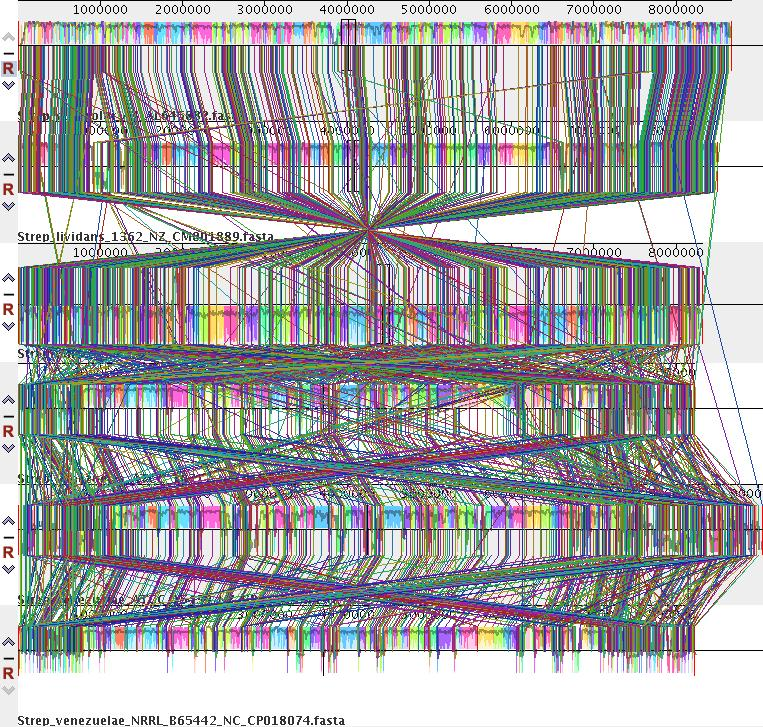
\includegraphics[width=\textwidth]{./figs/6_strep_strains_mauve_aln_pic}
		\caption{\label{fig:strep6mauvealn} Visualization of the \p alignment of 6 \strep genomes (from top to bottom): \scoe AL645882, \sliv NZ\_CM001889, \sliv NZ\_GG657756, \sven NC\_018750, \sven NZ\_CP013129, and \sven NC\_CP018074. Each coloured block represents a different locally co-linear block (LCB). Coloured lines connect LCBs that are similar btween taxa. The black lines underneath each LCB represent the whole genome sequence of each of the \strep taxa. Each LCB can be treated as a rearrangement, there have therefore been 521 rearrangements between these \strep genomes.}
	\end{center}
\end{figure}

	\begin{figure}[H]
	\begin{center}
		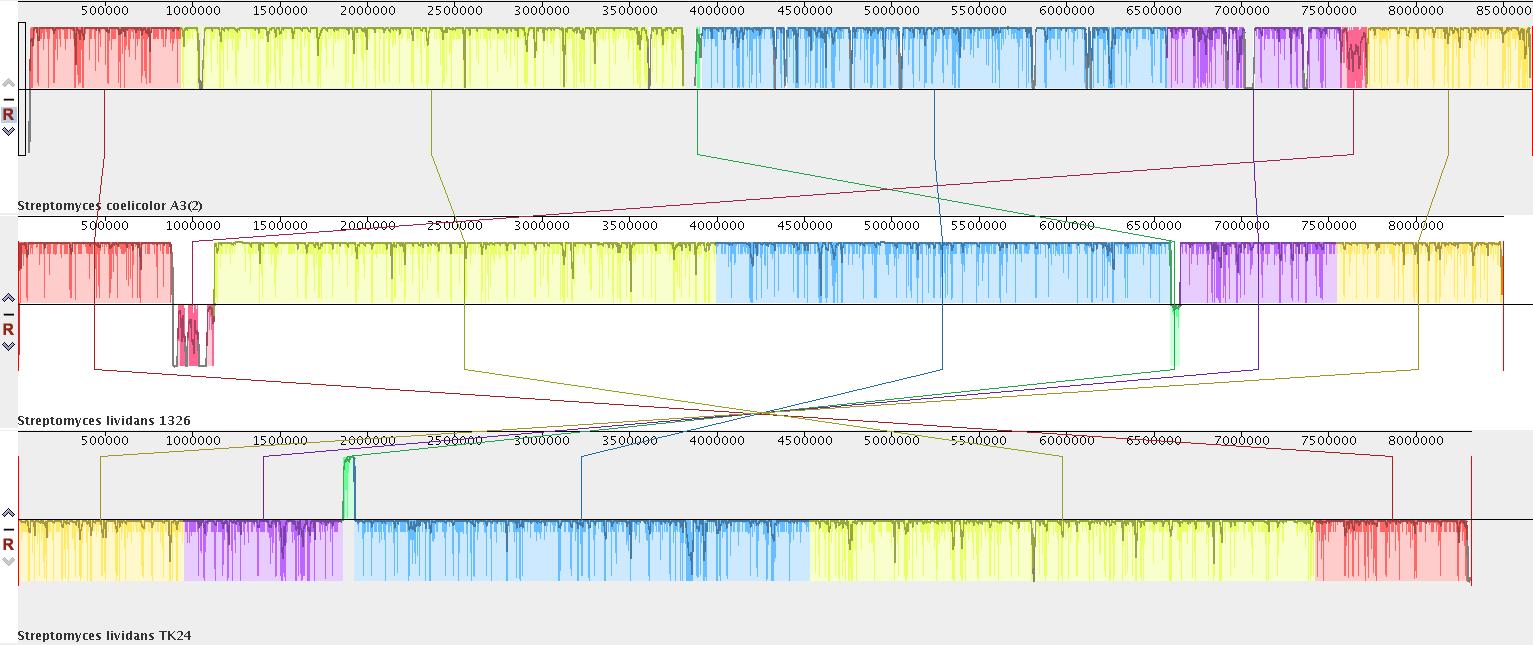
\includegraphics[width=\textwidth]{./figs/3_strep_strains_mauve_aln_pic}
		\caption{\label{fig:strep3mauvealn} Visualization of the \p alignment of the 3 \strep genomes chosen for this analysis (from top to bottom): \scoe AL645882, \sliv NZ\_CM001889, and \sliv NZ\_GG657756. Each coloured block represents a different locally co-linear block (LCB). Coloured lines connect LCBs that are similar btween taxa. The black lines underneath each LCB represent the whole genome sequence of each of the \strep taxa. Each LCB can be treated as a rearrangement, there have therefore been 6 rearrangements between these \strep genomes.}
	\end{center}
\end{figure}
	
	\begin{figure}[H]
	\begin{center}
		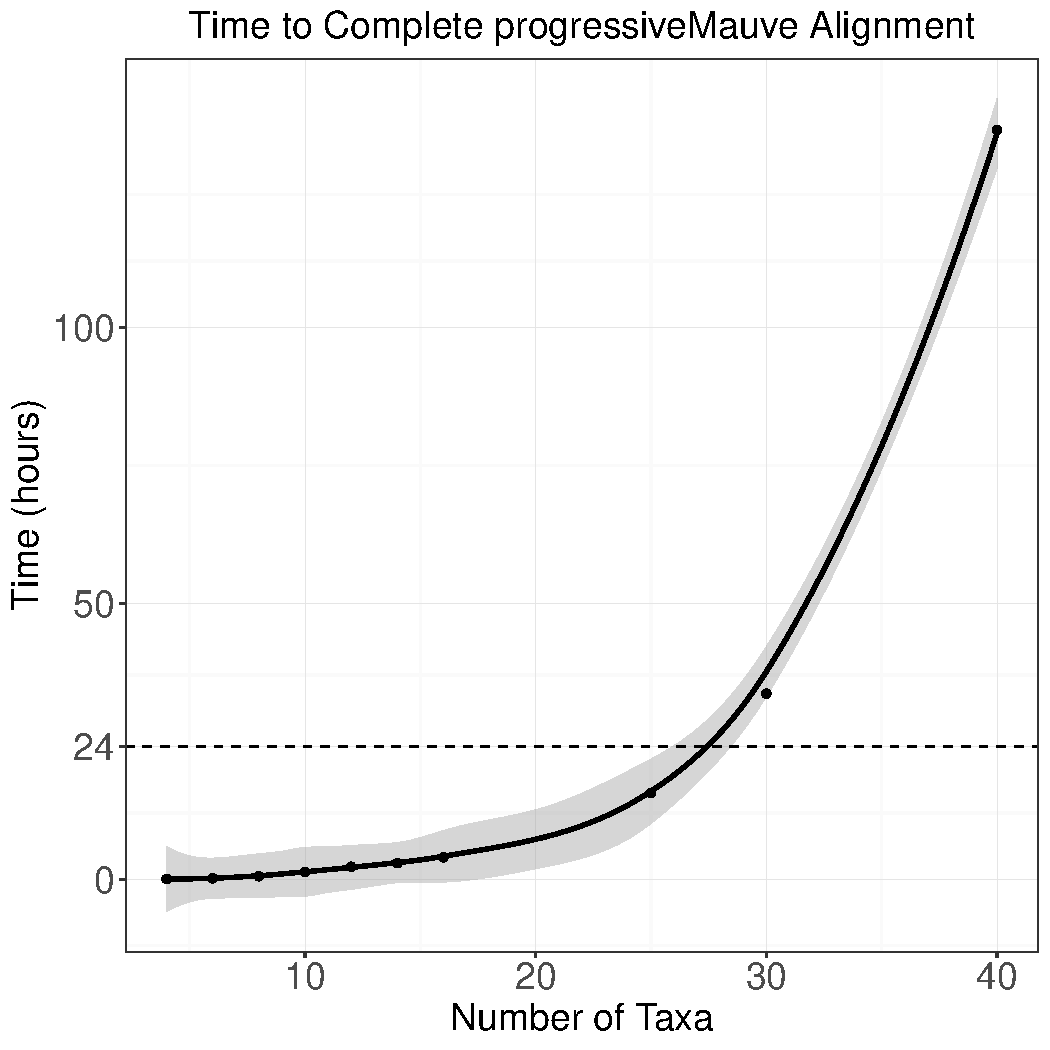
\includegraphics[width=0.51\textwidth]{./figs/mauve_time_plot}
		\caption{\label{fig:mauvetimeplot} This graph shows the time to complete a \p alignment with varying numbers of \ecol genomes. The total number of genomes or taxa is along the x-axis and the total time in hours is along the right axis. Each black point represents data from one \p alignment. All data points are connected by calculating locally estimated scatterplot smoothing (black line) with confidence intervals (grey band).}
	\end{center}
\end{figure}
	
	
	\subsection{\p Alignment}
	\begin{figure}[H]
		\begin{center}
			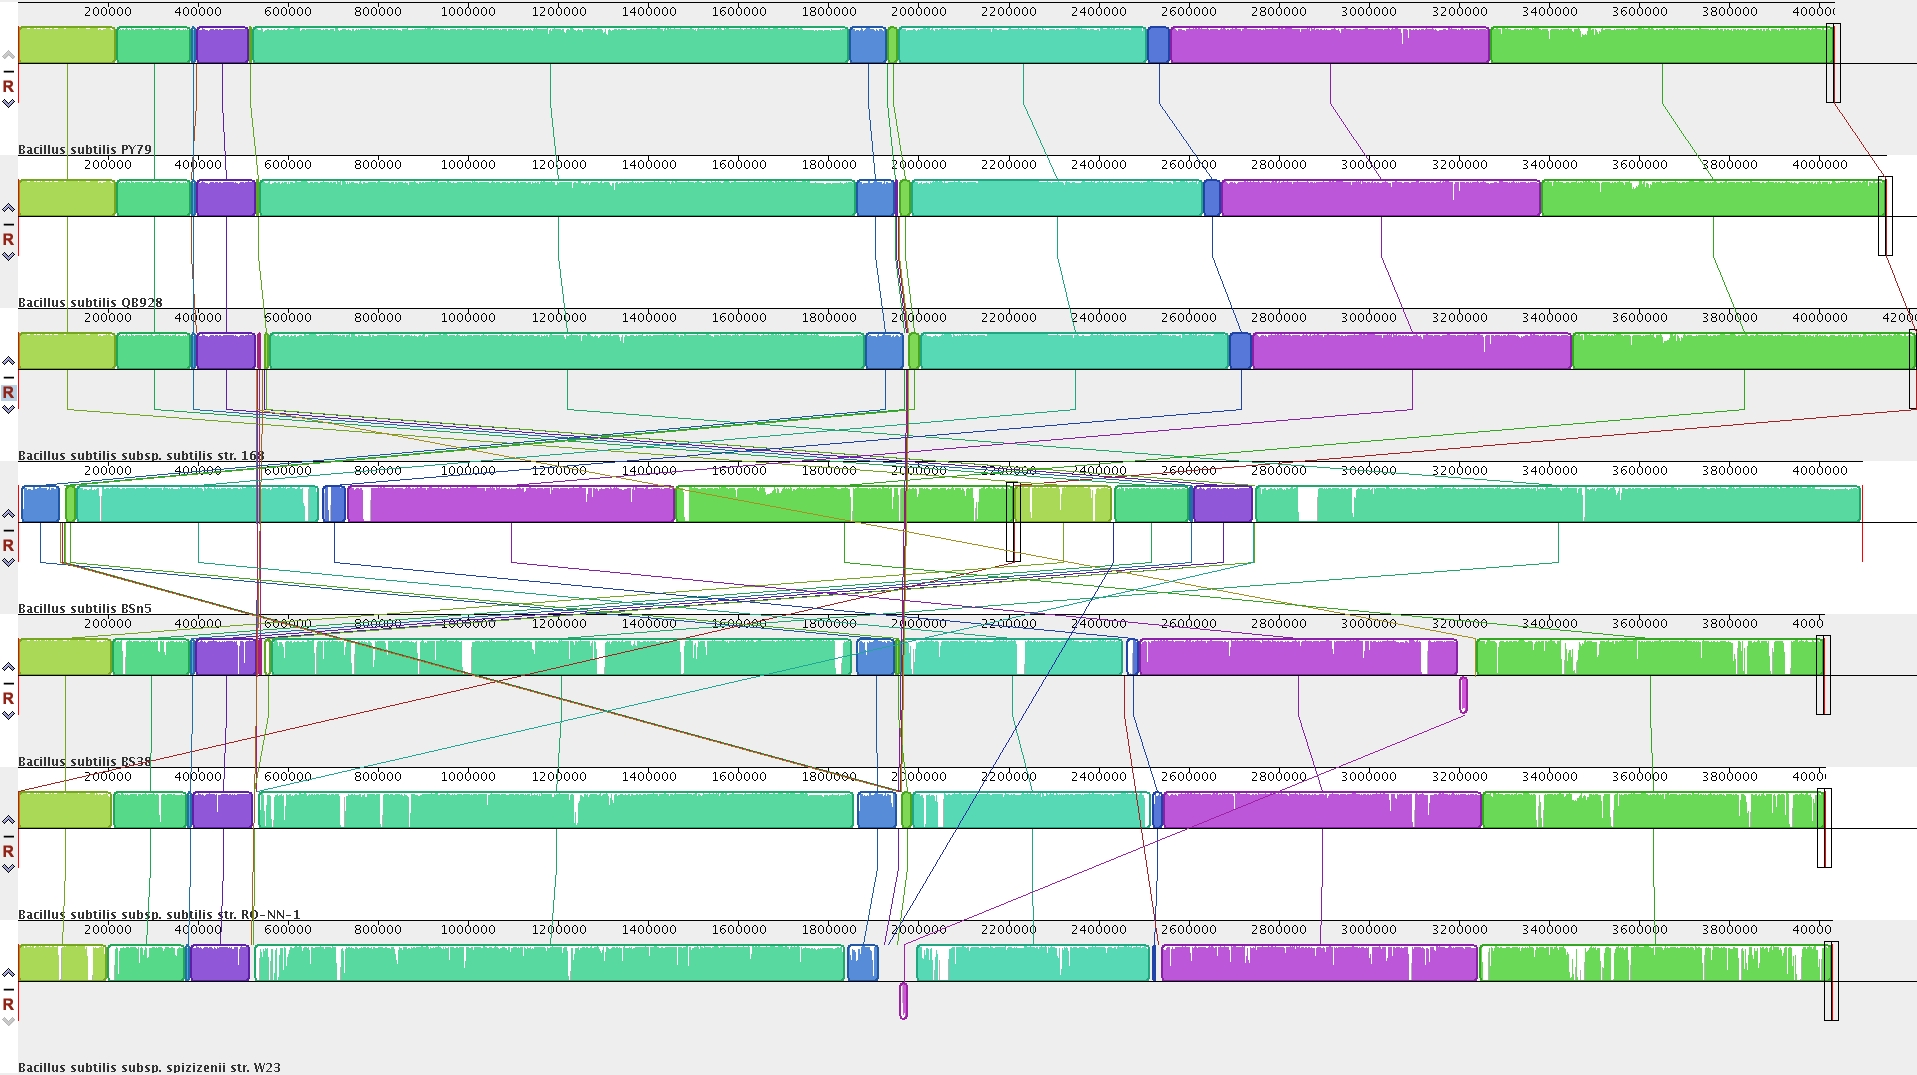
\includegraphics[width=\textwidth]{./figs/Bacillus_alignment_mauve.jpg}
			\caption{\label{fig:mauvealn} Visualization of the \p alignment of the \bass genomes. Each coloured block represents a different locally colinear block (LCB). Coloured lines connect LCBs that are similar btween taxa. The black lines underneath each LCB represent the whole genome sequence of each of the \bass taxa. From top to bottom the taxa are: \bass PY79, \bass QB928, \bass 168, \bass BSn5, \bass BS38, \bass RONN1, \bass W23.  Each LCB can be treated as a rearrangement, there have therefore been 12 rearrangements between these \bass genomes.}
		\end{center}
	\end{figure}

\subsection{Poor Sequence Alignment}
After a re-alignment of \p LCBs with \texttt{MAFFT} there were still regions of the alignment that were visibly poor.
This prompted the additional alignment quality trimming using a custom \texttt{Python} script and \texttt{trimAl} \citep{capella2009trimal}.
An example of what a ``poor'' alignment would look like can be found in Figure \ref{fig:ecoli_poor_aln}.
The \texttt{FASTA} format of this segment of the alignment can be found on \texttt{GitHub} labelled as file \texttt{``poor\_ecoli\_alignment\_example.fna''}.

This segment of \texttt{MAFFT} alignment (Figure \ref{fig:ecoli_poor_aln}) appears to have completely misaligned the second sequence (\ecol O157H7).
When we look at the genes that these regions of DNA are found within (Table \ref{tab:poor_aln_genes}), we see that the second sequence (\ecol O157H7) does not have the same protein sequence as the other bacteria genes.
Poor sequence alignments like this, as well as other non-homologous alignment regions were removed from the analysis.
Please see the main paper for more detailed methods.

	\begin{figure}[H]
	\begin{center}
		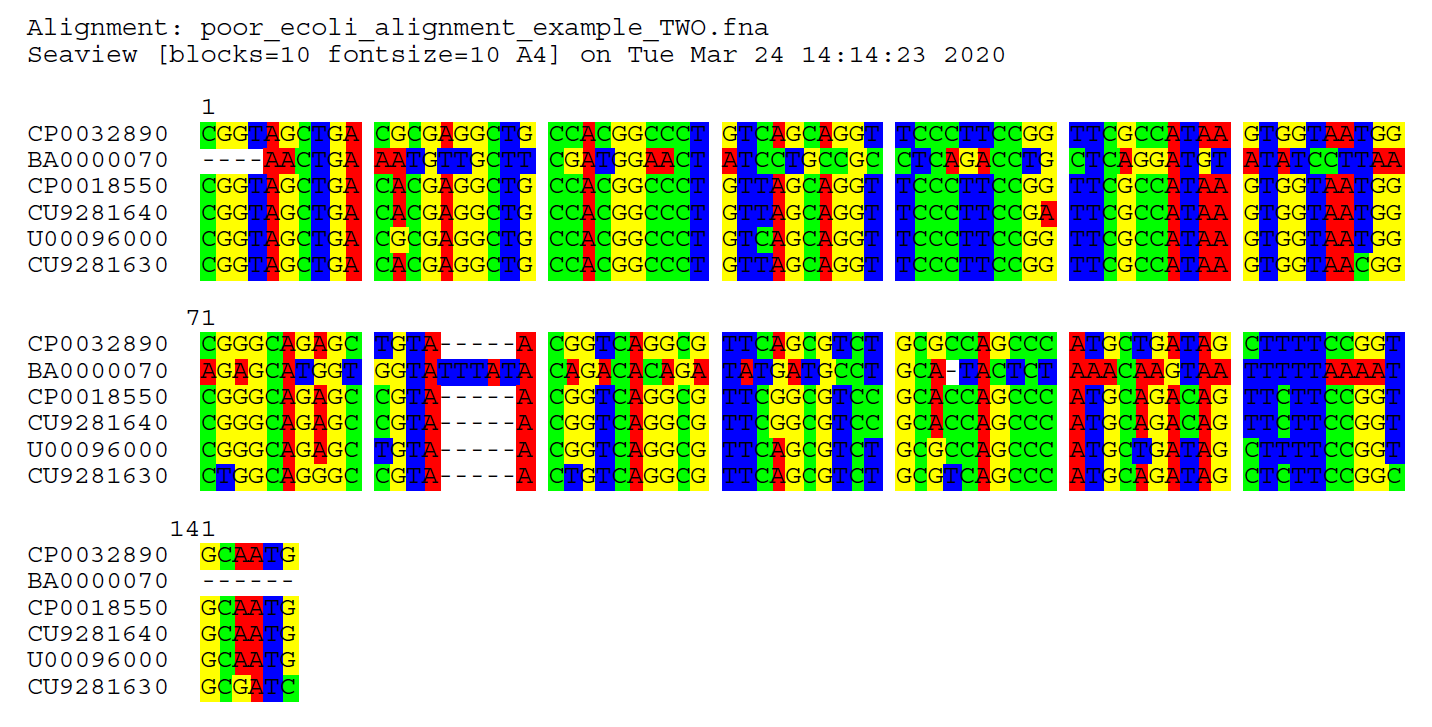
\includegraphics[width=0.9\textwidth]{./figs/Ecoli_poor_alignment_example.png}
		\caption{\label{fig:ecoli_poor_aln} Visualization of a section of \texttt{MAFFT} alignment between the six strains of \ecol. This alignment was visualized with the \texttt{SeaView} graphical interface \citep{Gouy:10}.}
	\end{center}
\end{figure}

	\begin{table}[H]
	\resizebox{\textwidth}{!}{%
		\begin{tabular}{lll}
			\toprule
			\ecol Strain & NCBI Accession Number & Alignment Gene Id \\  
			\midrule
			0104H4 & CP003289 & O3K\_04155\\
		    O157H7 & BA000007 & ECs3861\\
			083H1 & CP001855&  NRG857\_18350\\
			IAI39 & CU928164& yghE\\
			K12 & U00096& yghE\\
			UMN026 & CU928163& yghE\\
			\bottomrule
		\end{tabular}
	}%resize box
	\caption{\label{tab:poor_aln_genes} \ecol strain, NCBI accession number, and Gene Id for the genes in the poor alignment example (Figure \ref{fig:ecoli_poor_aln}).}
\end{table}

	
	\subsection{Phylogenetic Trees}
	\begin{figure}[H]
		\begin{center}
			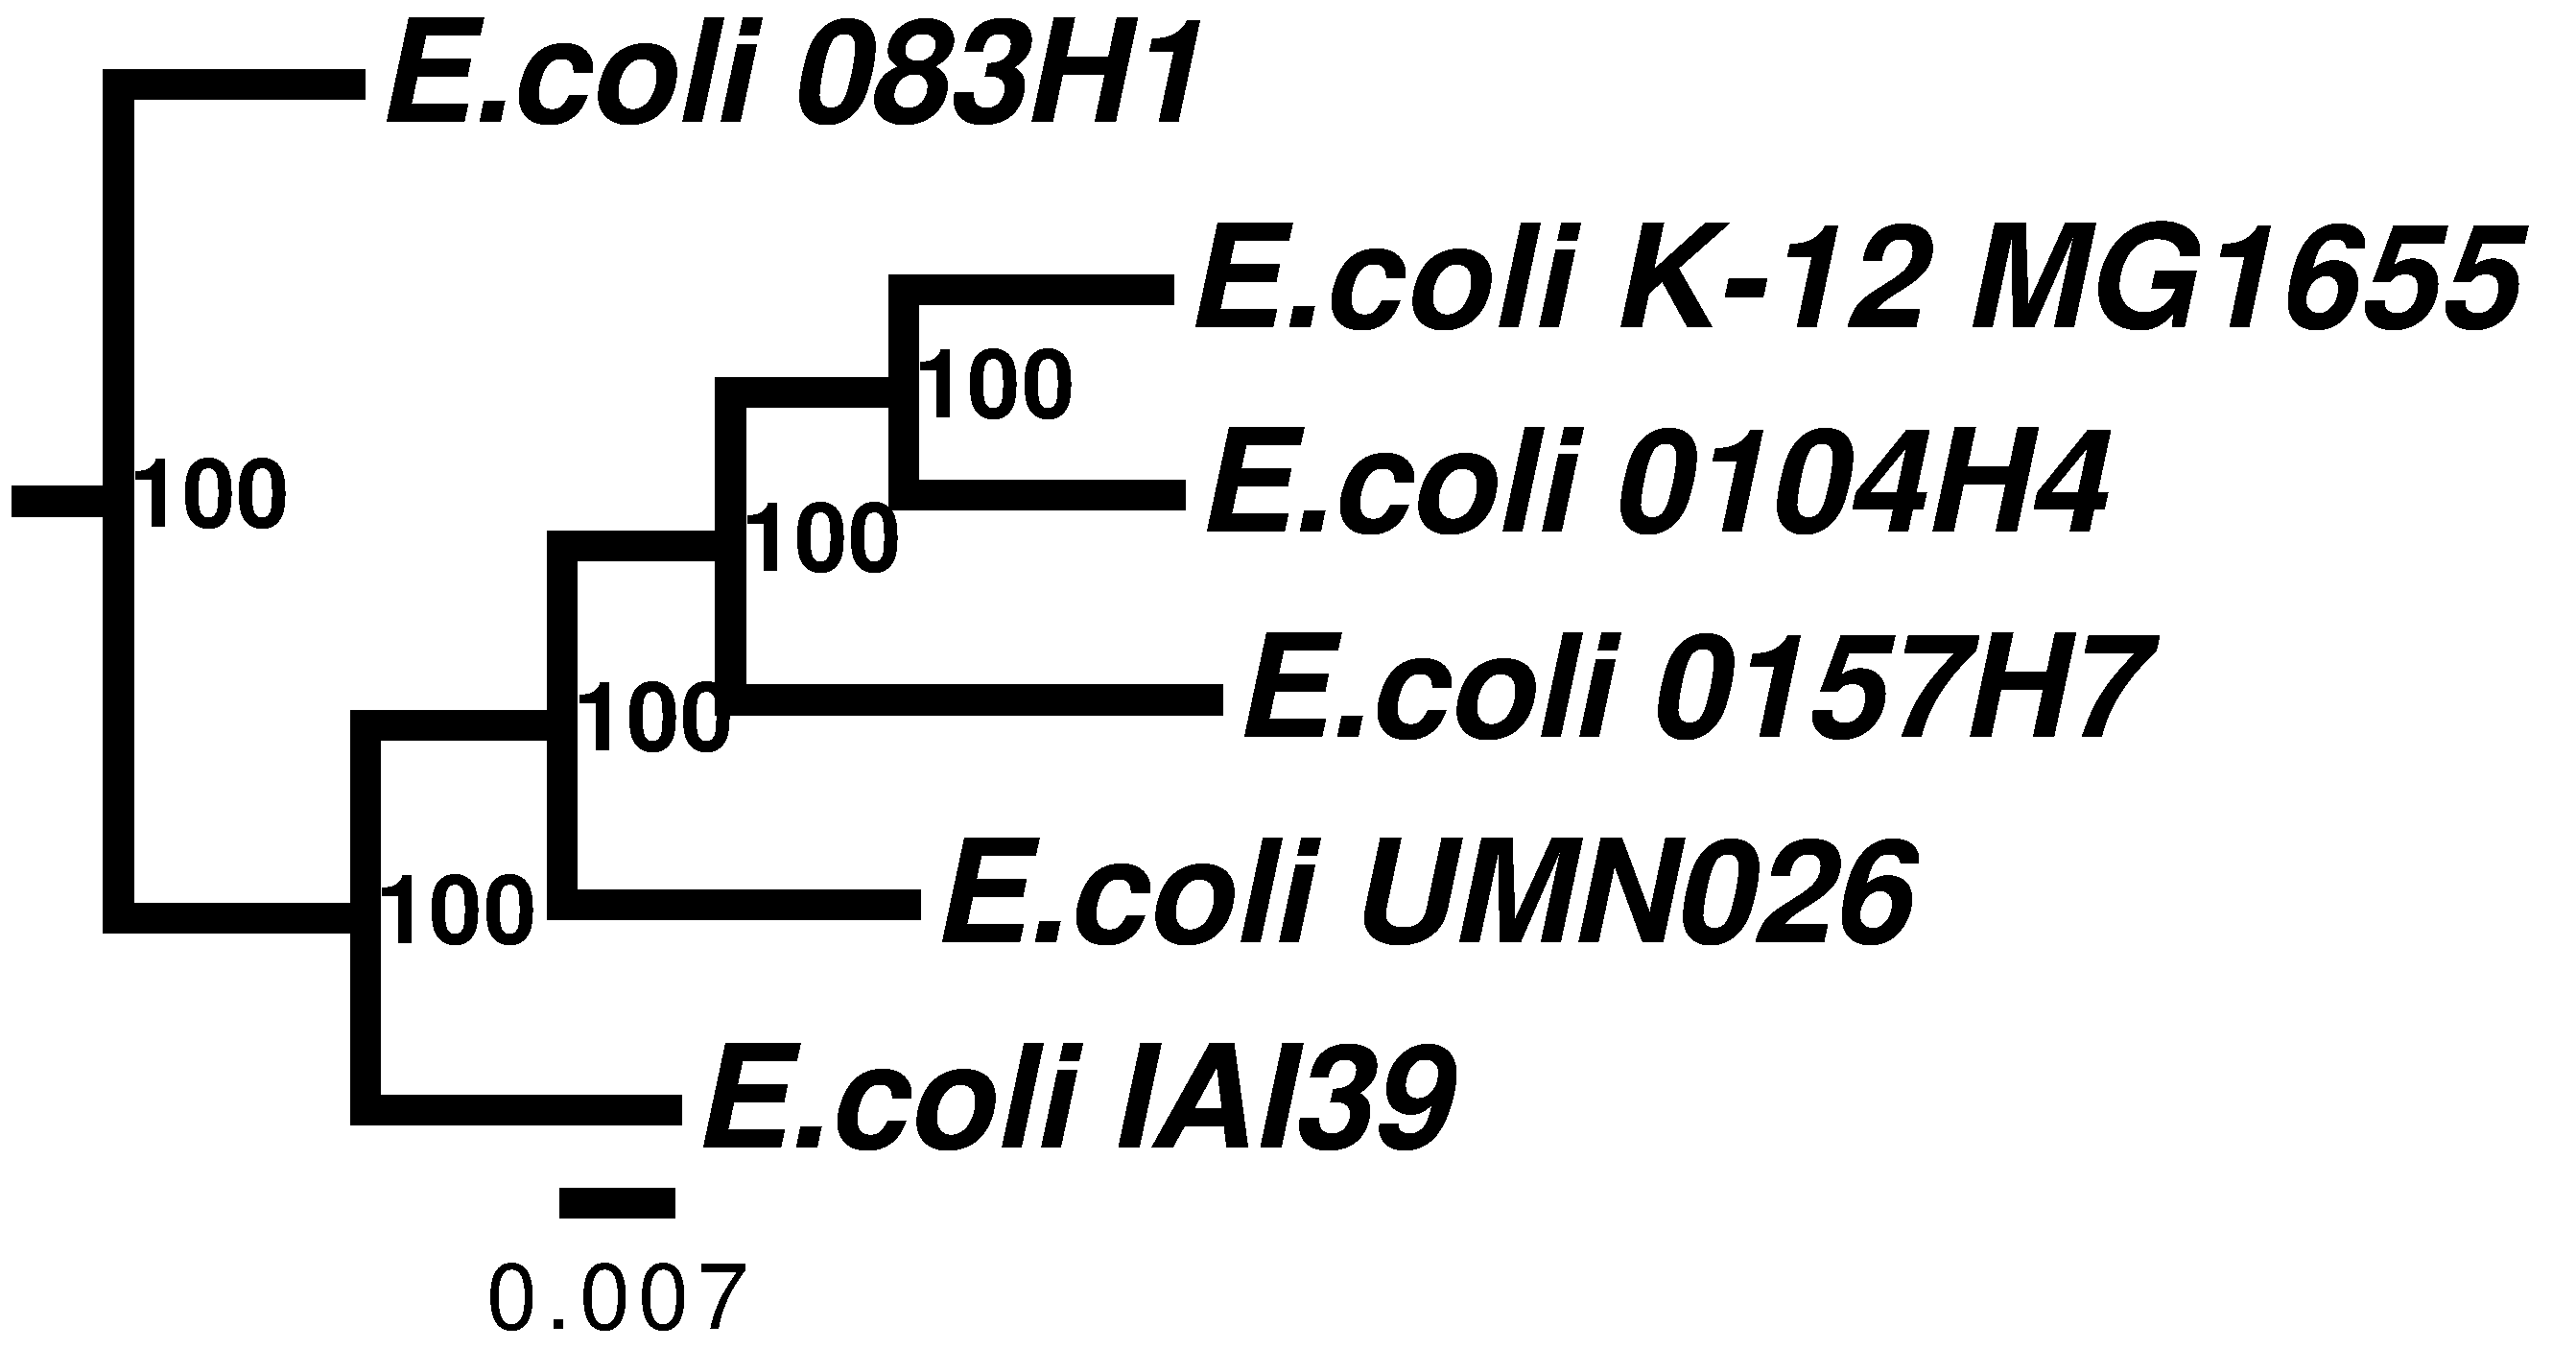
\includegraphics[width=0.7\textwidth]{./figs/Ecoli_chrom_ref_tree_figtree_raw_29Aug20.pdf}
			\caption{\label{fig:ecolitree} Phylogenetic tree of \ecol genomes. \salm was used as an outgroup to root the tree. Branch lengths are to scale. The numbers at each node indicate the bootstrap value as a percentage. The number of bootstrapped trees was 100.}
		\end{center}
	\vspace*{\floatsep}% http://tex.stackexchange.com/q/26521/5764
	
		\begin{center}
			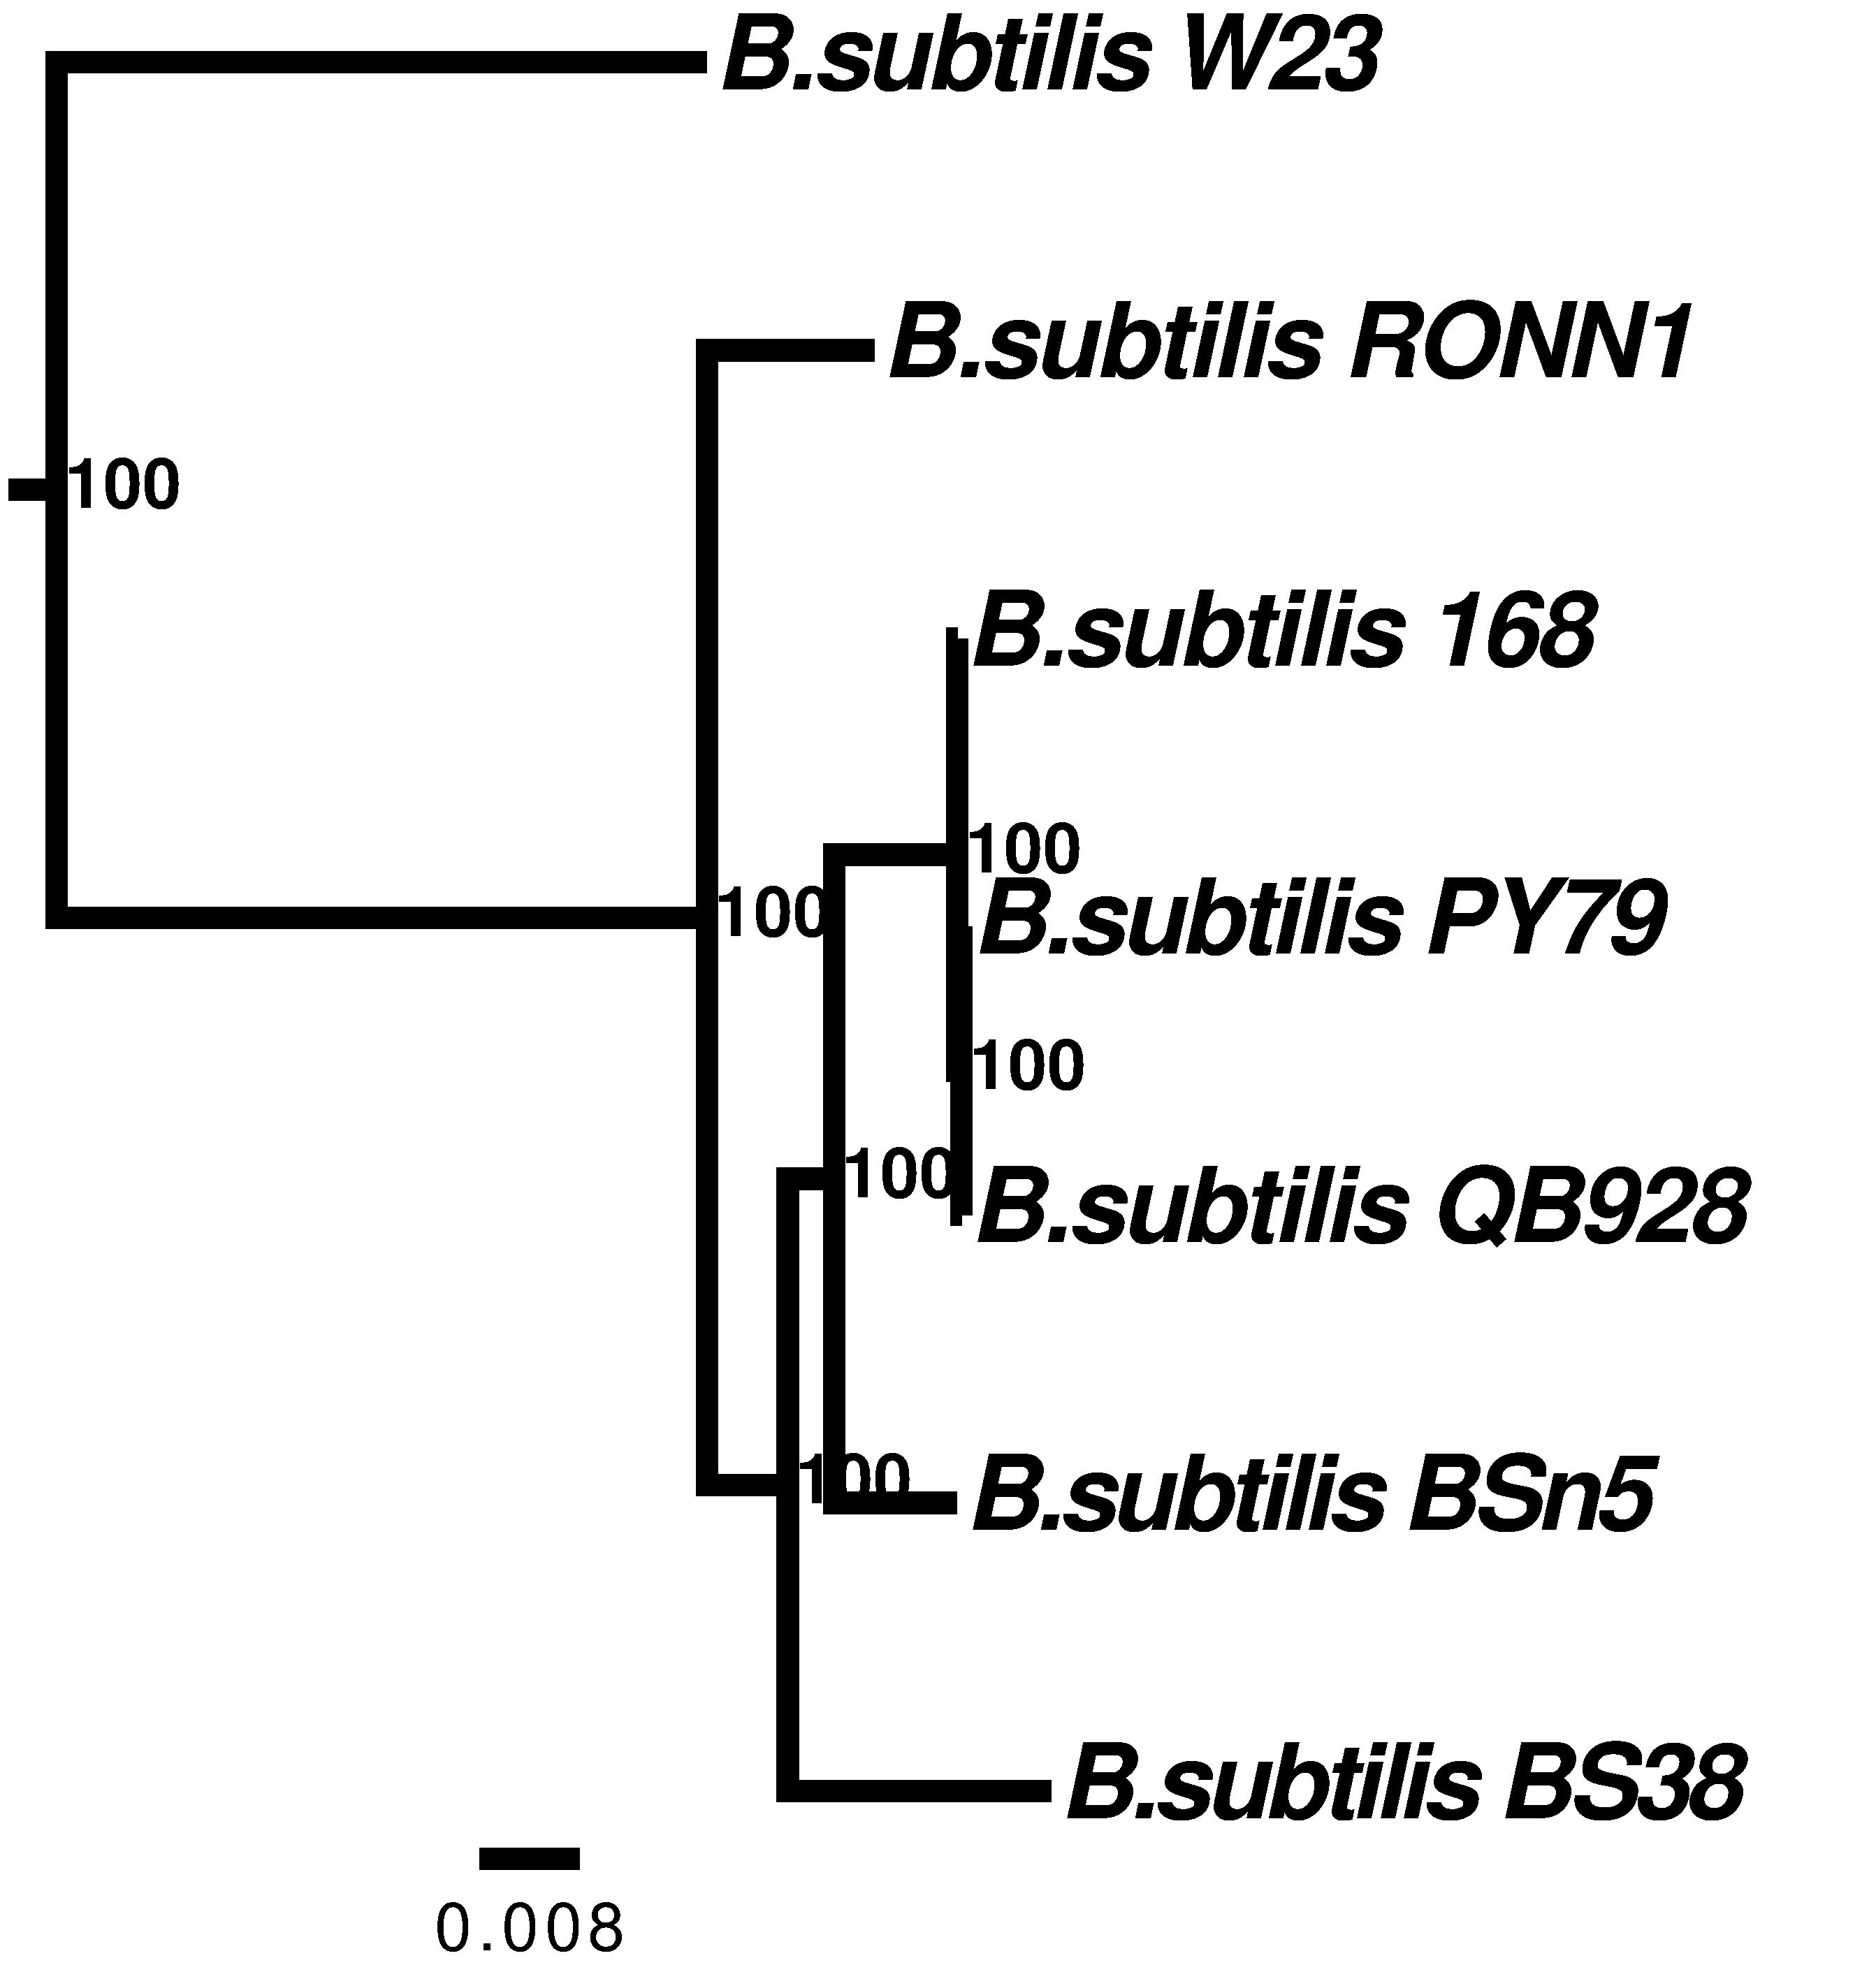
\includegraphics[width=0.7\textwidth]{./figs/bass_chrom_ref_tree_figtree_raw_29Aug20.pdf}
			\caption{\label{fig:basstree} Phylogenetic tree of \bass genomes. \lis was used as an outgroup to root the tree. Branch lengths are to scale. The numbers at each node indicate the bootstrap value as a percentage. The number of bootstrapped trees was 100.}
		\end{center}
			
		\end{figure}
		
		\begin{figure}[H]
		\begin{center}
			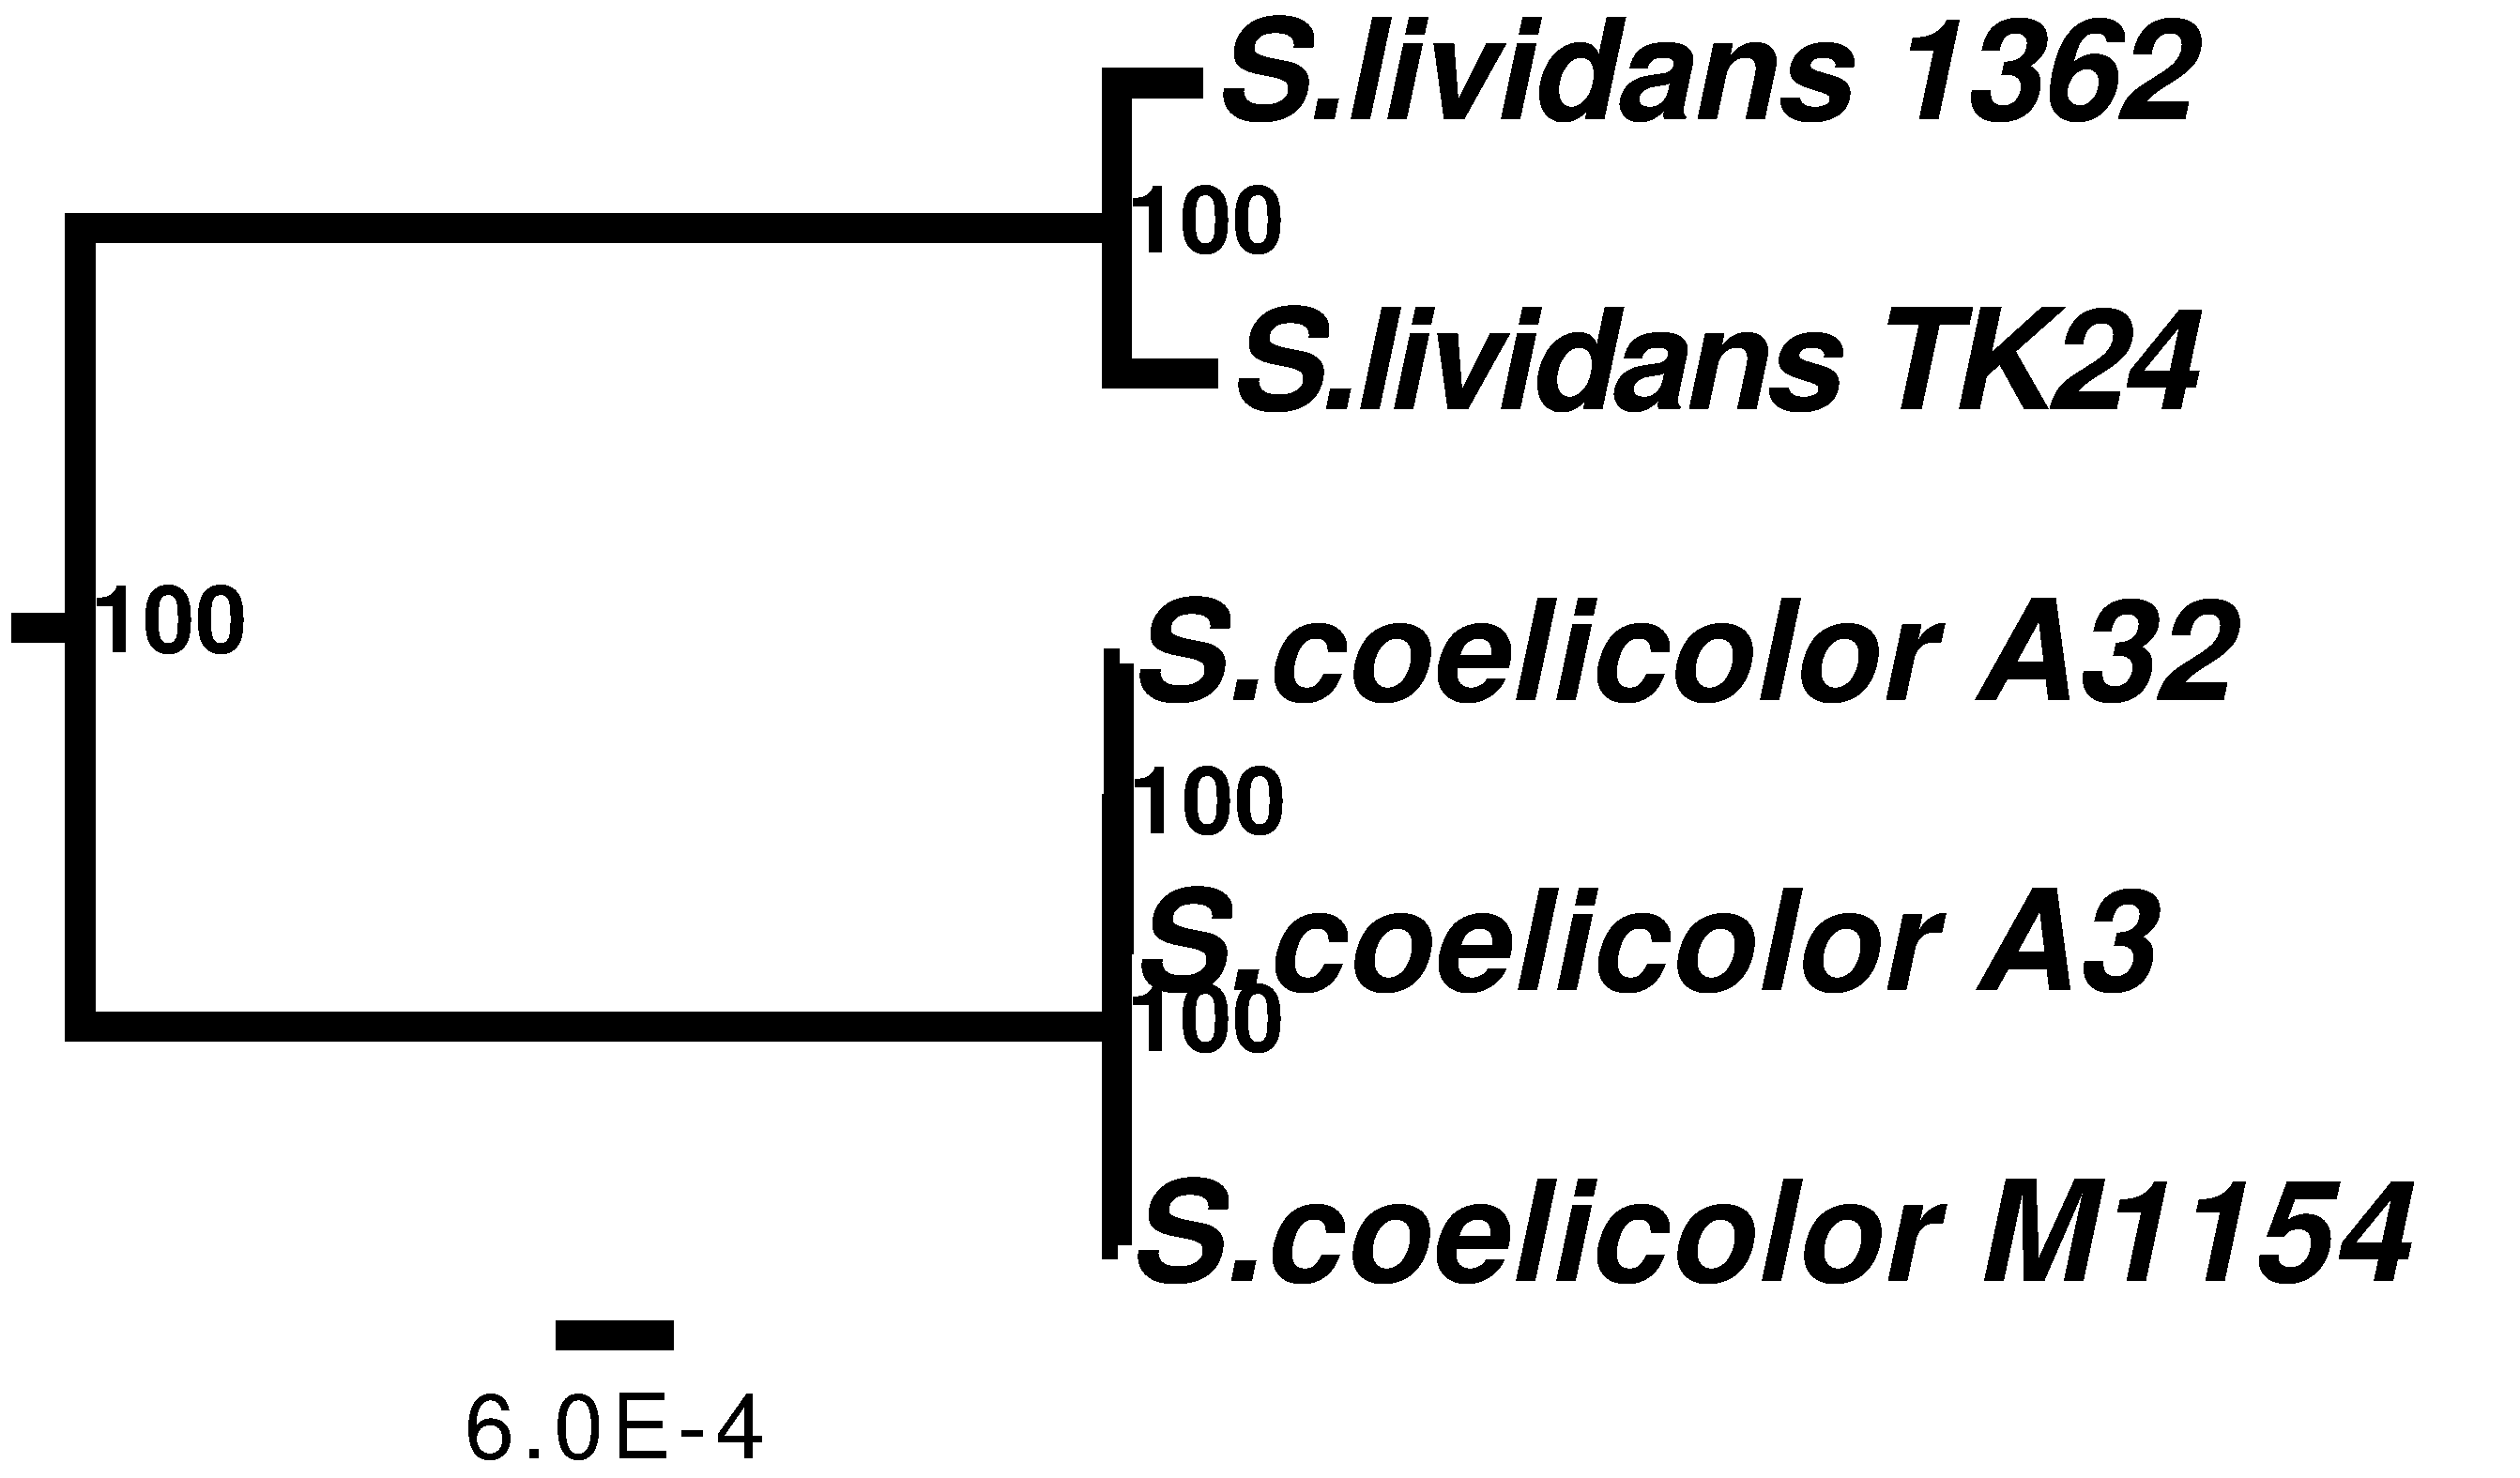
\includegraphics[width=0.7\textwidth]{./figs/Strep_chrom_figtree_raw_11Sep20.pdf}
			\caption{\label{fig:streptree} Phylogenetic tree of \strep genomes. \tub was used as an outgroup to root the tree. Branch lengths are to scale. The numbers at each node indicate the bootstrap value as a percentage. The number of bootstrapped trees was 100.}
		\end{center}
			\vspace*{\floatsep}% http://tex.stackexchange.com/q/26521/5764
		\begin{center}
			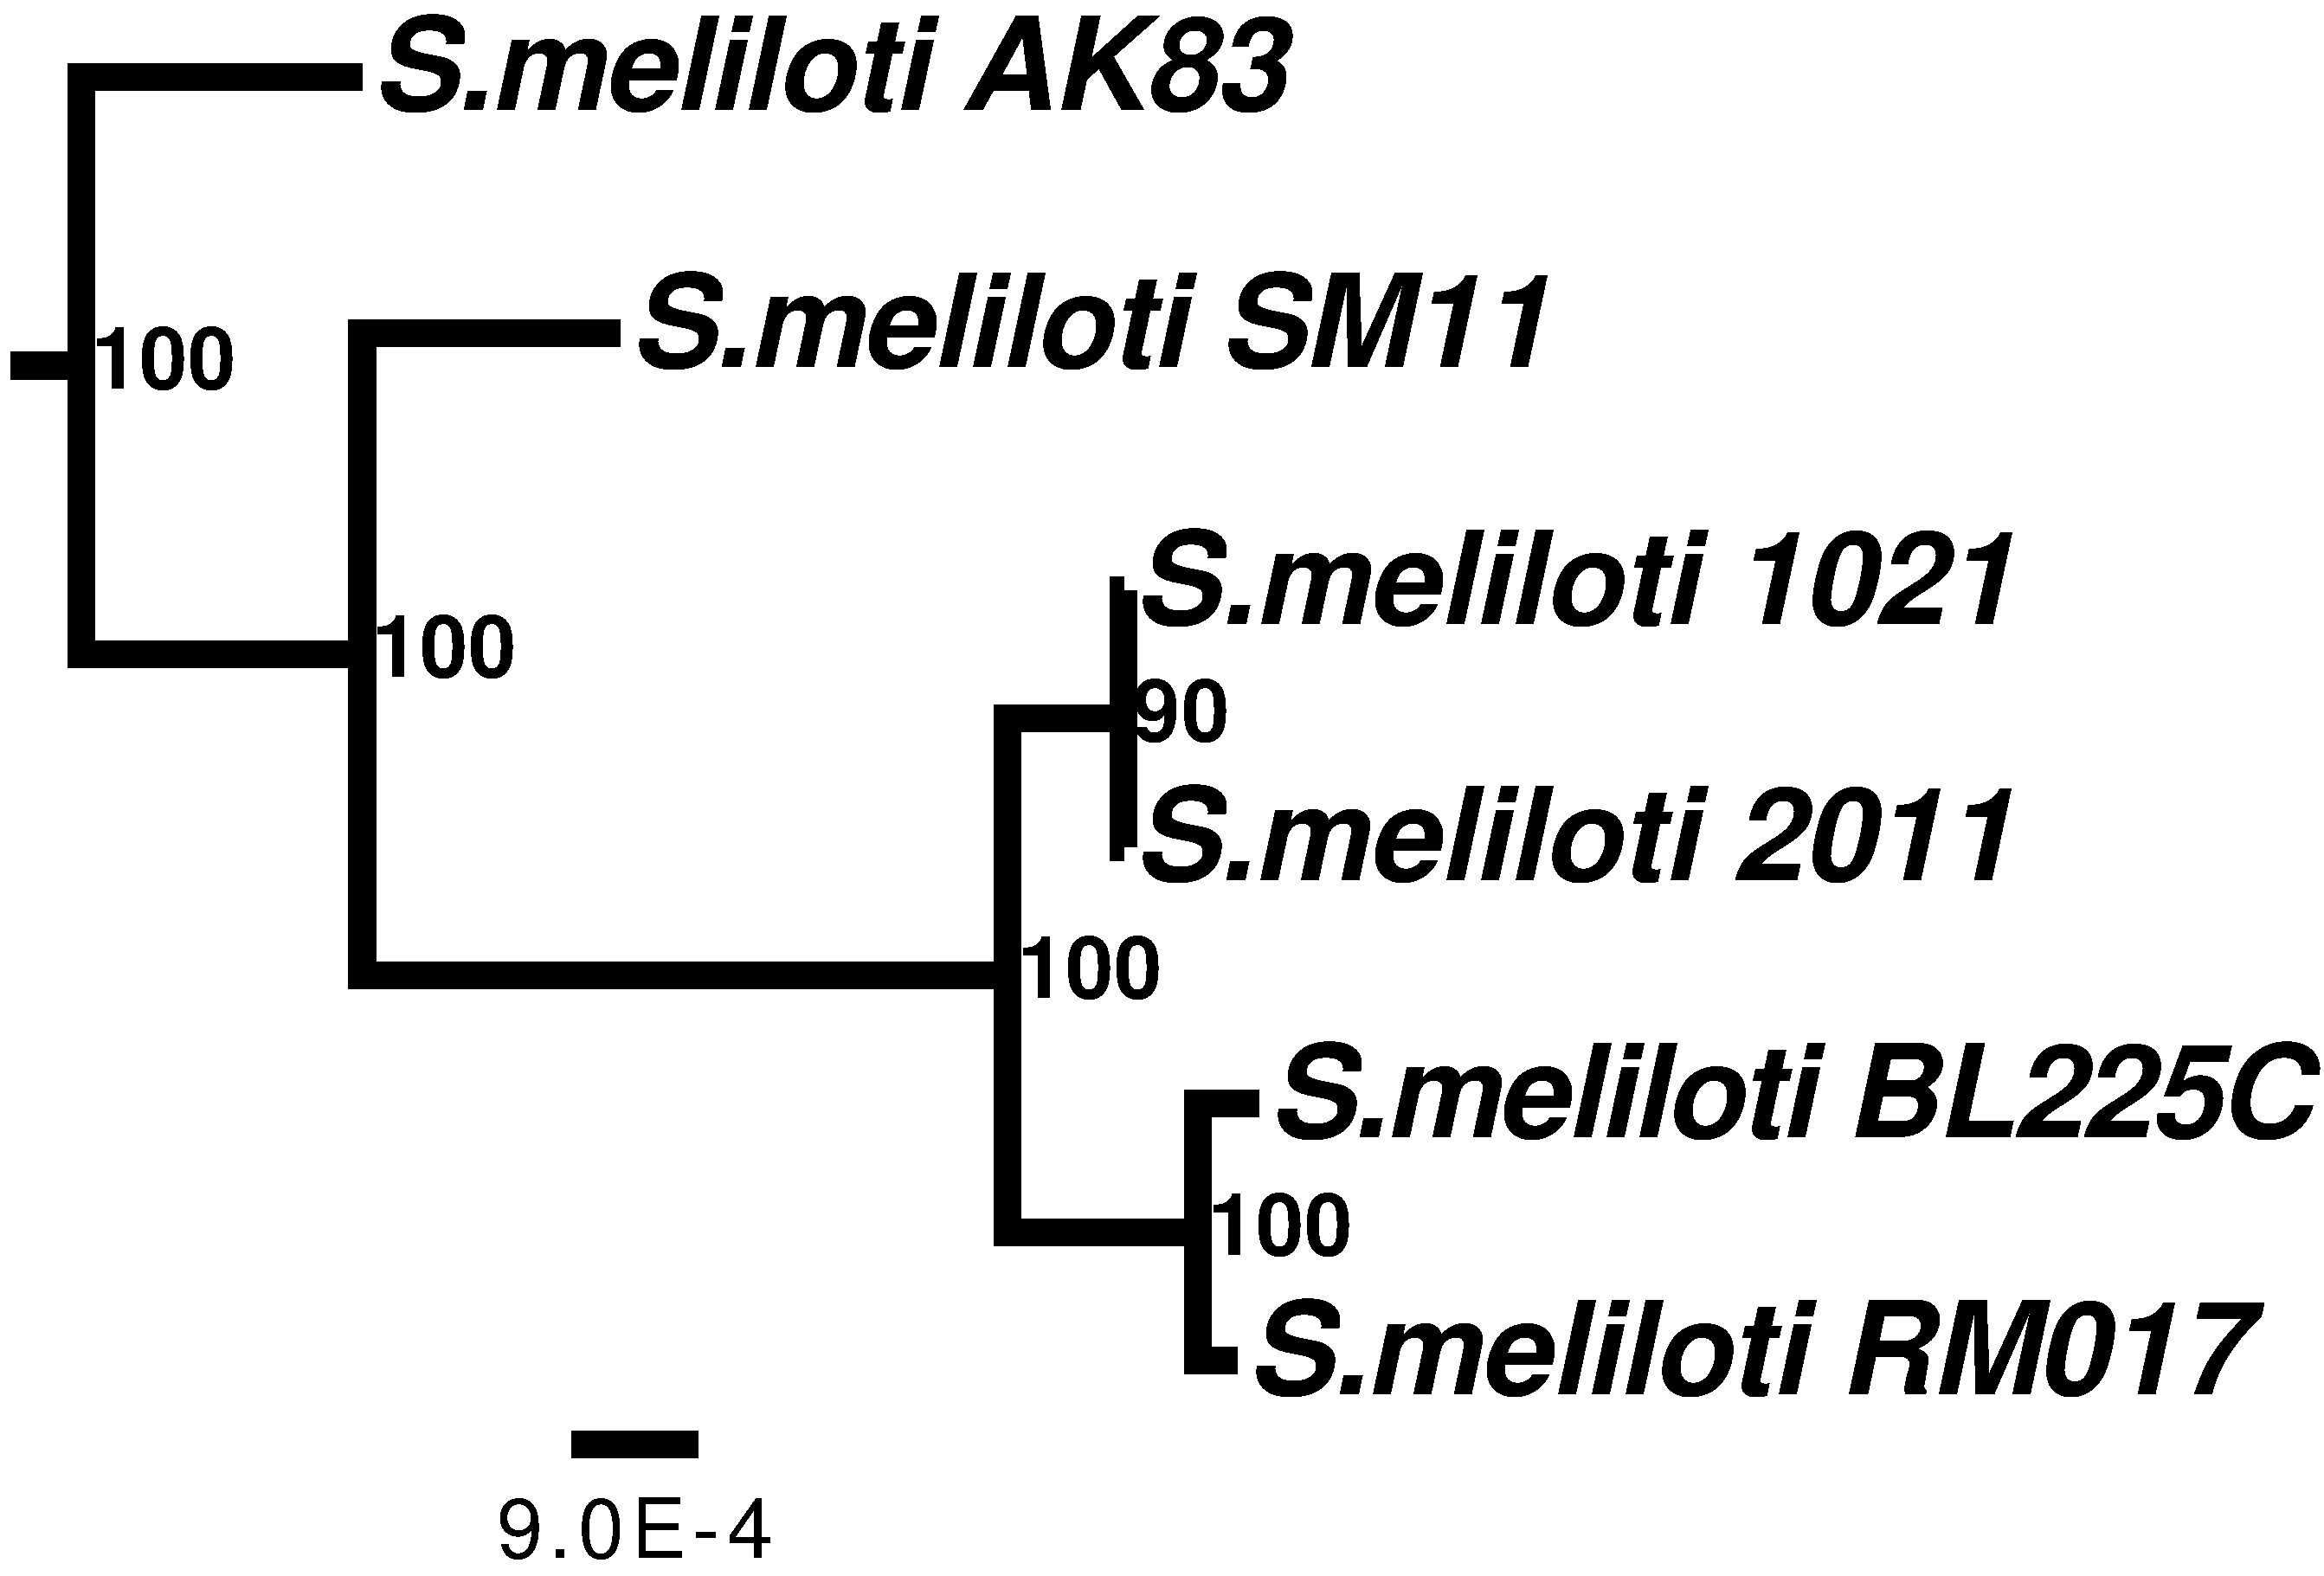
\includegraphics[width=0.7\textwidth]{./figs/SinoC_chrom_figtree_raw_11Sep20.pdf}
			\caption{\label{fig:sinoCtree} Phylogenetic tree using only the chromosomes of \smel. \agro circular chromosome was used as an outgroup to root the tree. Branch lengths are to scale. The numbers at each node indicate the bootstrap value as a percentage. The number of bootstrapped trees was 100.}
		\end{center}
	\end{figure}
		
		\begin{figure}
		\begin{center}
			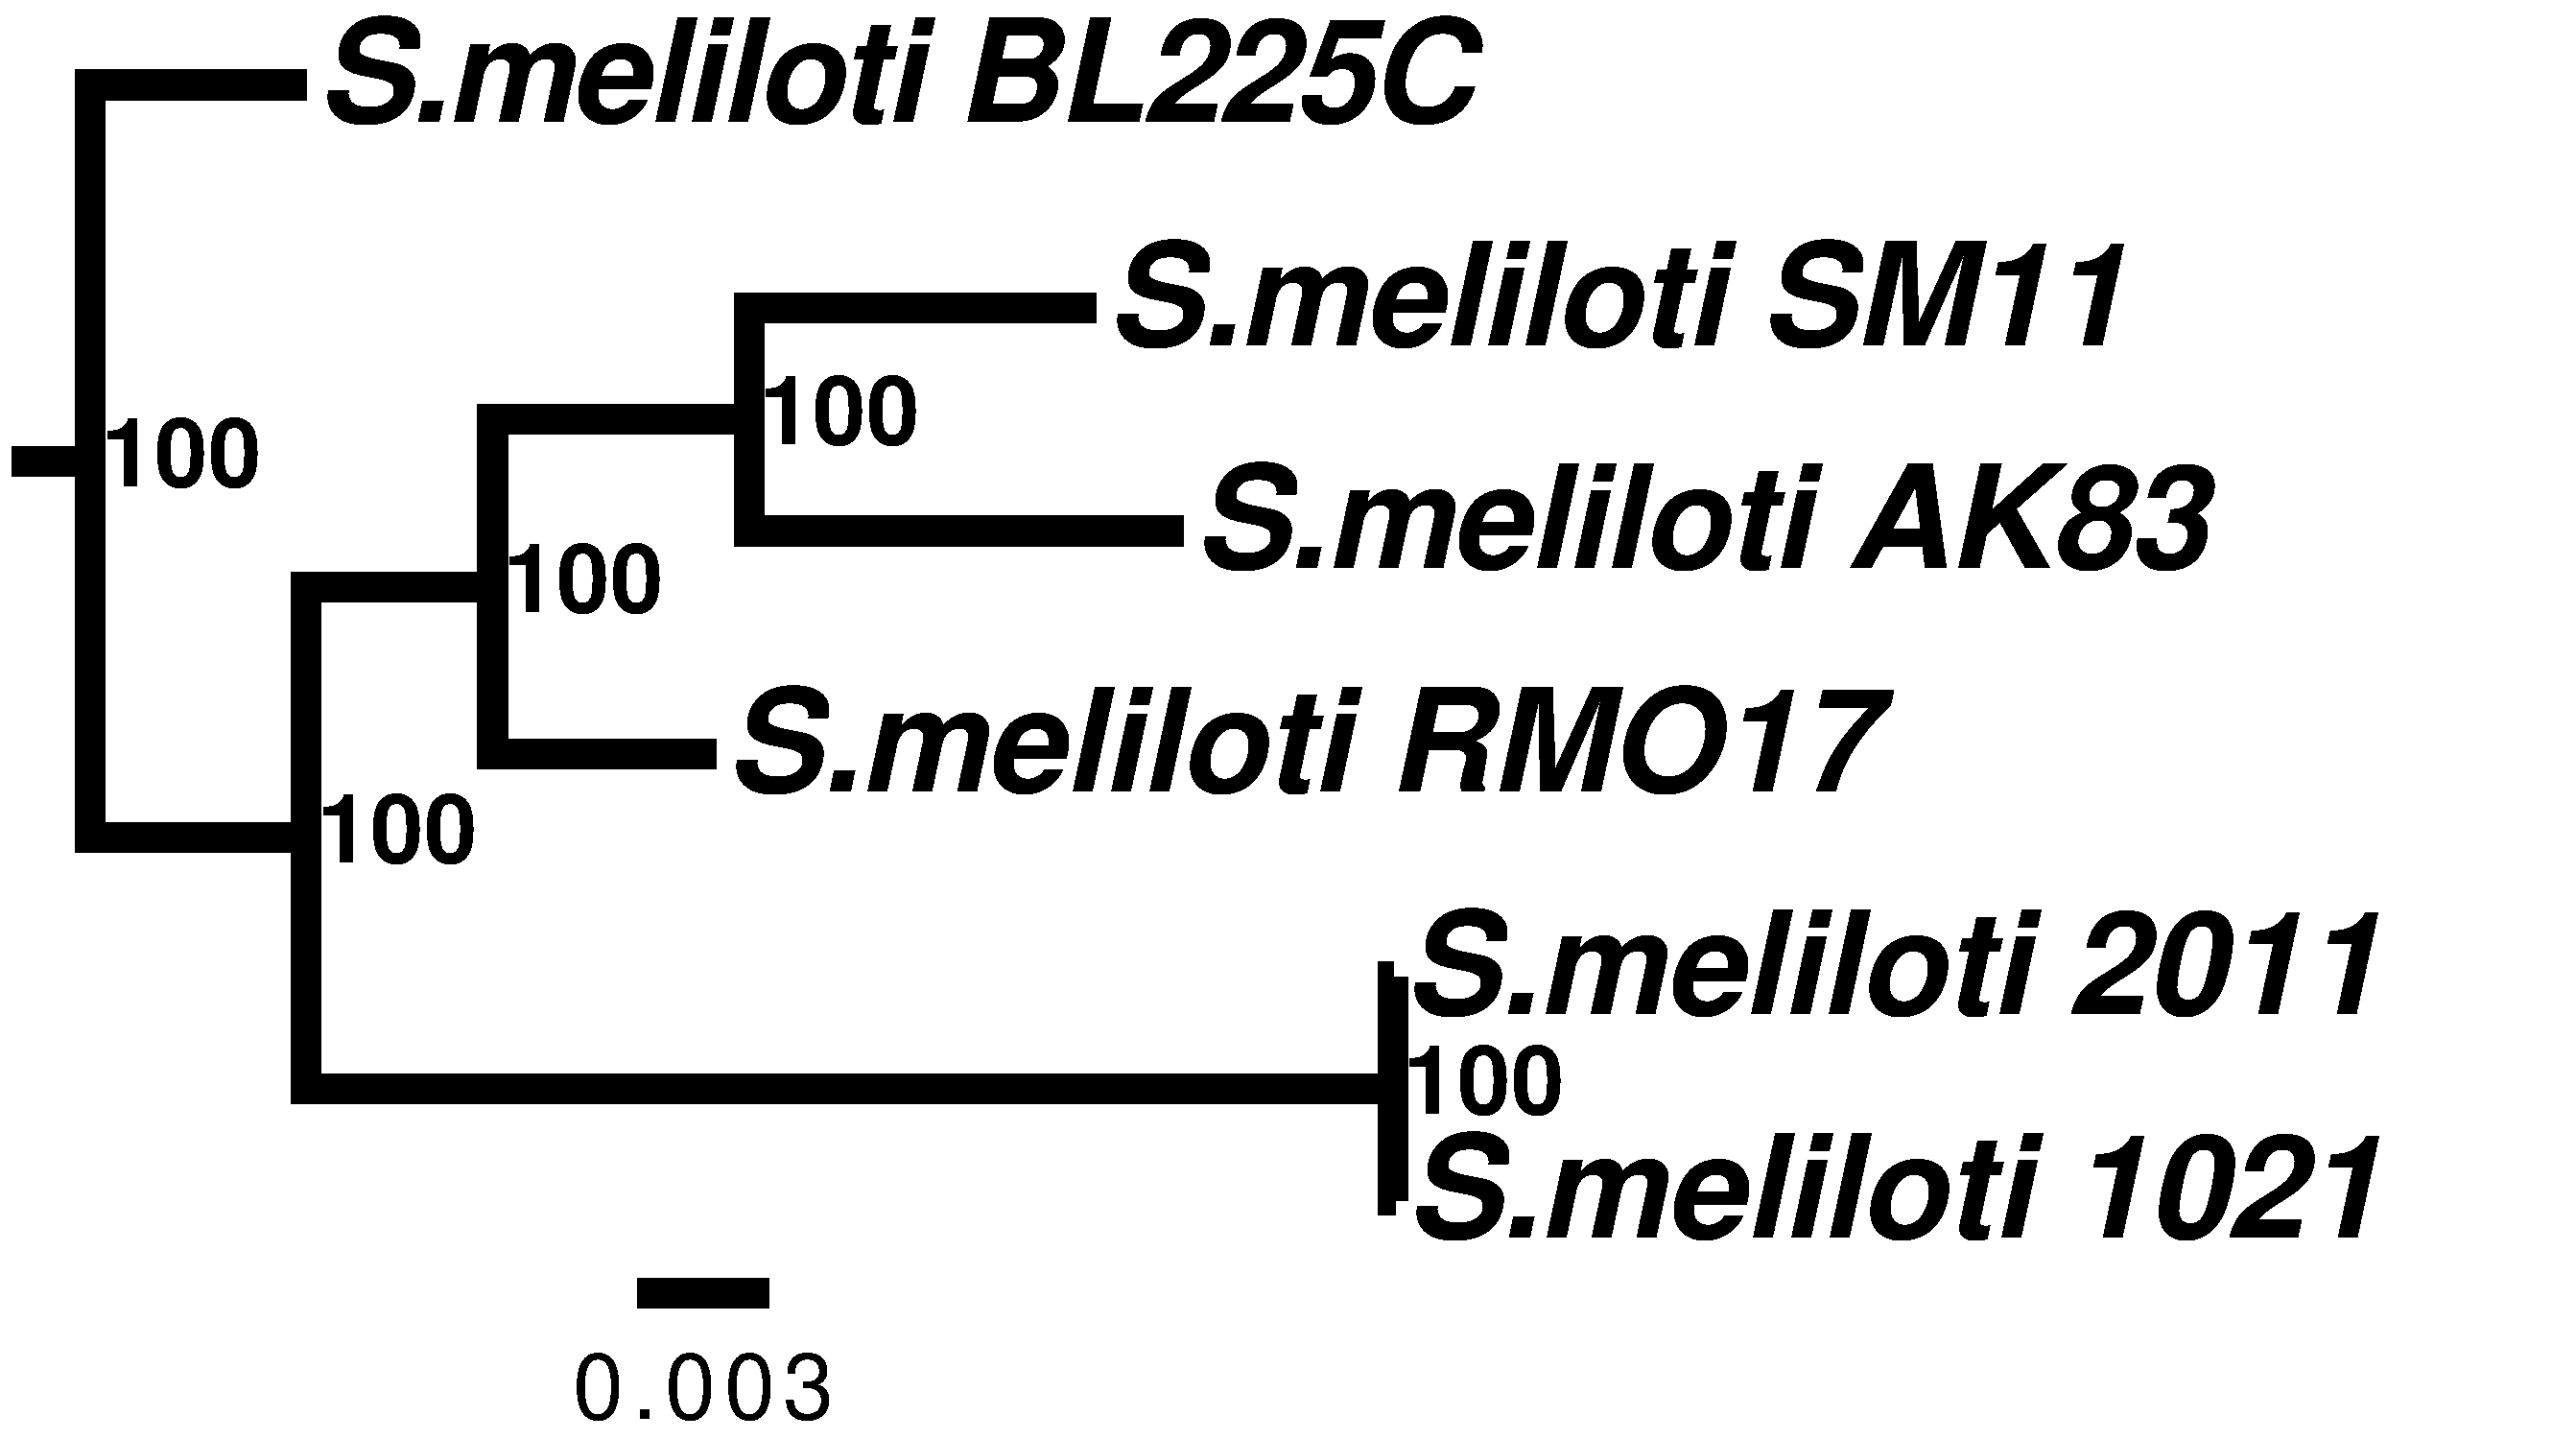
\includegraphics[width=0.7\textwidth]{./figs/pSymA_chrom_figtree_raw_29Aug20.pdf}
			\caption{\label{fig:sinoPAtree} Phylogenetic tree using only pSymA of \smel. \agro circular plasmid was used as an outgroup to root the tree. Branch lengths are to scale. The numbers at each node indicate the bootstrap value as a percentage. The number of bootstrapped trees was 100.}
		\end{center}
		\vspace*{\floatsep}% http://tex.stackexchange.com/q/26521/5764
			\begin{center}
				
				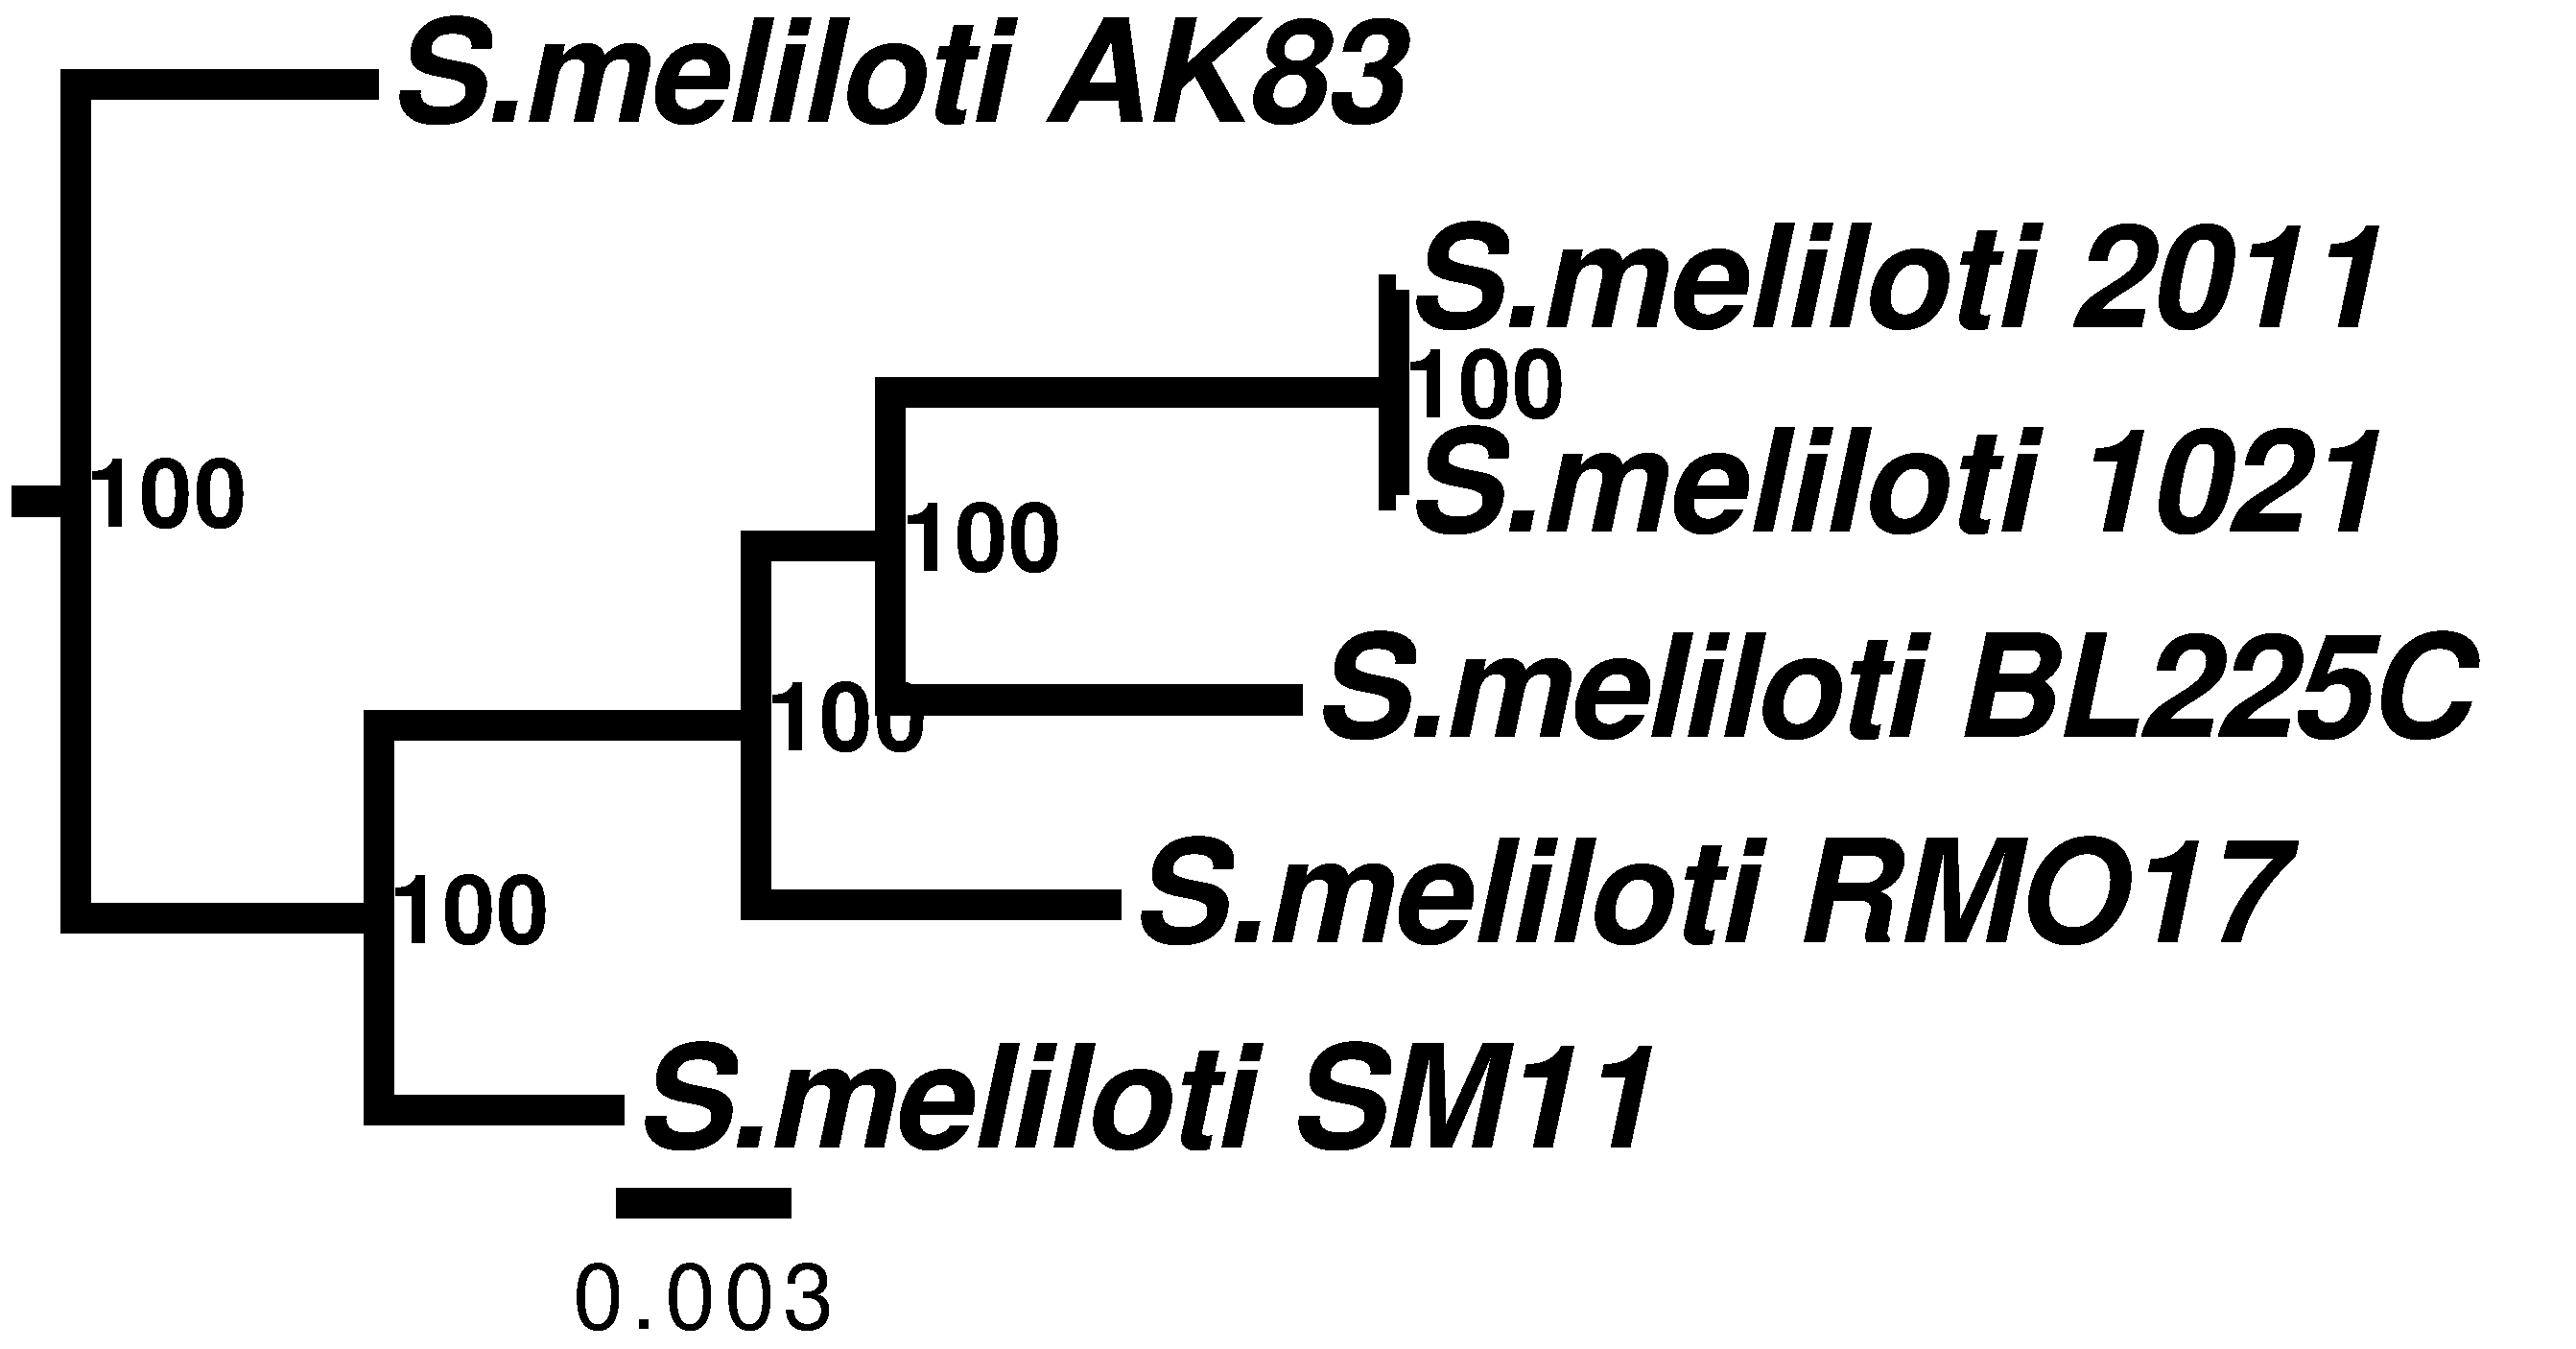
\includegraphics[width=0.7\textwidth]{./figs/pSymB_chrom_figtree_raw_29Aug20.pdf}
				\caption{\label{fig:sinoPBtree} Phylogenetic tree using only pSymB of \smel. \agro circular chromid was used as an outgroup to root the tree. Branch lengths are to scale. The numbers at each node indicate the bootstrap value as a percentage. The number of bootstrapped trees was 100.}
			\end{center}
		\end{figure}
	
	
	\begin{table}[H]
		\resizebox{\textwidth}{!}{%
			\begin{tabular}{lccc}
				\toprule
				Bacteria Replicon & \multicolumn{1}{p{3cm}}{\centering \# of Total LCBs \\ with Identical Tree} & 
				\multicolumn{1}{p{3cm}}{\centering \# of Total LCBs \\ with Non- identical Tree} & 
				\multicolumn{1}{p{3cm}}{\centering \% of Total Alignment Discarded} \\  
				\midrule
				\ecol Chromosome & 30 & 7 & 25.44\%\\
				\bass Chromosome & 10 & 2 & 21.62\%\\
				\strep Chromosome & NA & NA & NA\\
				\smel Chromosome & 9 & 2 & 25.06\%\\
				\smel \pa & 35 & 0 & 0\%\\
				\smel \pb & 8 & 0 & 0\%\\
				\bottomrule
			\end{tabular}
		}%resize box
		\caption{\label{fig:treetopresults} Number of Locally Colinear Blocks that had identical topologies to the ``super sequence'' tree, not identical to the ``super sequence'' tree, and the proportion of the total alignment that was represented by the non-identical tree topologies. Topologies that were not identical were determined to be different at the 5\% significant value using an SH-test in \texttt{RAxML} \citep{stamatakis2014raxml}. The SH-Test could not be preformed on \strep as there were only three taxa present and \texttt{RAxML} needs a minimum of 4 taxa for the test  \citep{stamatakis2014raxml}.}
	\end{table}
	
	\subsection{Origin and Terminus Locations}

Each of the bacterial strains used in this analysis vary in total genomic length, in some cases this difference is up to 856Kbp like in \ecol (Table \ref{tab:oriloc}). 
This will cause the farthest point from the origin of replication to appear larger because of the increased genome size of some strains.


	\begin{table}[H]
		\begin{center}
			\begin{tabular}{lccc}
				\toprule
				Bacteria & Origin of Replication & Terminus of Replication & Length of Longest Genome (bp)\\
				\midrule
				\ecol & 3925744 & 1588773 & 5498450 \\
				\bass & 1 & 1942542 & 4215606\\
				\strep & 3419363 & 1 \& 8667664 & 8667664\\
				\smel Chromosome & 1 & 1735626 & 3908022\\
				\smel pSymA & 1350001 & 672888 & 1633319\\
				\smel pSymB & 55090 & 896756 & 1690594\\
				\bottomrule
			\end{tabular}
			\caption{\label{tab:oriloc} Origin of replication and terminus of replication positions in replicons of \ecol, \bass, \strep, and \smel. The origin and terminus of replication are values from the representative strain of each bacteria, which can be found in Supplementary Table \ref{tab:seqdata}. The linear nature of \strep chromosome gives it two termini, one at each end of the chromosome. The lenght of the longest genome is the longest genome length from all strains/species of each bactiera. This is not necessarally the same as the genome length of the representative strain.}
		\end{center}
	\end{table}
	
		\begin{table}[H]
			\centering
			\resizebox{\textwidth}{!}{%
				\begin{tabular}{lcccccc}
					\toprule
					Origin Location & \ecol Chromosome &\bass Chromosome & \strep Chromosome & \smel Chromosome &\smel pSymA & \smel pSymB\\
					\midrule
					Moved 100kb Left & -1.445\e{-7}*** & 4.374\e{-9}* &  6.909\e{-9}*** &  -1.316\e{-6}*** & -1.058\e{-6}*** & -2.009\e{-7}***\\
					Moved 90kb Left & -1.544\e{-7}*** & -1.036\e{-7}*** & 5.677\e{-9}*** & -1.32\e{-6}*** & -1.246\e{-6}*** &-1.357\e{-7}***\\
					Moved 80kb Left& -1.65\e{-7}*** & -1.072\e{-7}*** & 8.11\e{-9}*** & -1.338\e{-6}*** & -1.398\e{-6}*** & -6.57\e{-8}***\\
					Moved 70kb Left& -1.667\e{-7}*** & -1.102\e{-7}*** & 6.716\e{-9}*** & -1.363\e{-6}*** & -1.405\e{-6}*** & 9.83\e{-8}\\
					Moved 60kb Left& -1.64\e{-7}*** & -1.19\e{-7}*** & 8.7\e{-9}*** & -1.324\e{-6}*** & -1.394\e{-6}*** & 1.129\e{-7}***\\
					Moved 50kb Left& -1.446\e{-7}*** & -1.211\e{-7}*** & 1.045\e{-8}*** & -1.36\e{-6}*** & -1.403\e{-6}*** & 1.521\e{-7}***\\
					Moved 40kb Left& -1.4\e{-7}*** & -1.299\e{-7}*** & 1.214\e{-8}*** & -1.255\e{-6}*** & -1.422\e{-6}*** & 1.543\e{-7}***\\
					Moved 30kb Left& -1.498\e{-7}*** & -1.292\e{-7}*** & 1.24\e{-8}*** & -1.26\e{-6}*** & -1.392\e{-6}*** & 1.63\e{-7}***\\
					Moved 20kb Left& -1.51\e{-7}*** & -1.1\e{-7}*** & 1.395\e{-8}*** & -1.525\e{-6}*** & -1.412\e{-6}*** & 1.603\e{-7}***\\
					Moved 10kb Left& -1.262\e{-7}*** & -2.602\e{-9} & 1.563\e{-8}*** &  -1.599\e{-6}*** &  -9.499\e{-7}*** & 2.973\e{-7}*** \\
					Moved 10kb Right& -1.305\e{-7}*** & -2.045\e{-8}*** & 1.578\e{-8}*** & 1.614\e{-6}*** & -1.026\e{-6}*** & 3.505\e{-7}*** \\
					Moved 20kb Right& -1.454\e{-7}*** & -1.006\e{-7}*** & 1.903\e{-8}*** & -1.634\e{-6}*** & -1.475\e{-6}*** & 1.649\e{-7}***\\
					Moved 30kb Right& -1.548\e{-7}*** & -8.596\e{-8}*** & 2.046\e{-8}*** & -1.698\e{-6}*** & -1.417\e{-6}*** & 1.526\e{-7}***\\
					Moved 40kb Right& -1.632\e{-7}*** & -8.378\e{-8}*** & 2.125\e{-8}*** & -1.719\e{-6}*** & -1.367\e{-6}*** & 1.589\e{-7}***\\
					Moved 50kb Right& -1.856\e{-7}*** & -7.879\e{-8}*** & 1.957\e{-8}*** & -1.735\e{-6}*** & -1.277\e{-6}*** & 1.654\e{-7}***\\
					Moved 60kb Right& -1.91\e{-7}*** & -6.98\e{-8}*** & 1.974\e{-8}*** & -1.788\e{-6}*** & -1.169\e{-6}*** & 1.645\e{-7}***\\
					Moved 70kb Right& -1.892\e{-7}*** & -6.634\e{-8}*** & 1.934\e{-8}*** & -1.854\e{-6}*** & -1.059\e{-6}*** & 1.843\e{-7}***\\
					Moved 80kb Right& -1.879\e{-7}** & -5.814\e{-8}*** & 2.313\e{-8}*** & -1.891\e{-6}*** & -9.07\e{-7}*** & 1.90\e{-7}***\\
					Moved 90kb Right& -1.862\e{-7}*** & -4.314\e{-8}*** & 2.304\e{-8}*** & -1.865\e{-6}*** & -7.171\e{-7}*** & 2.415\e{-7}***\\
					Moved 100kb Right& -1.799\e{-7}*** & -2.597\e{-8}*** &  1.945\e{-8}*** &  -1.525\e{-6}*** & -6.572\e{-7}*** & 3.095\e{-7}***\\
					\bottomrule
				\end{tabular}
				
			}%resizebox
				\caption{\label{tab:orishuffel} Logistic regression analysis of the number of substitutions along the genome of the respective bacterial replicons after the origin location was moved by the specified increments from the original origin of replication position (listed in Table \ref{tab:oriloc}). All results are marked with significance codes as followed: $<$ 0.001 = `***', 0.001 $<$ 0.01 = `**', 0.01 $<$ 0.05 = `*', 0.05 $<$ 0.1 = `.', $>$ 0.1 = ` '. Logistic regression was calculated after the origin of replication was moved to the new location in the genome and all subsequent positions were scaled around the origin accounting for bidirectionality of replication.}
		\end{table}
		
\begin{table}[H]
			\centering
			\resizebox{\textwidth}{!}{\begin{minipage}{\textwidth}
					\begin{tabular}{lll}
						\toprule
						Bacteria Strain & Accession Number & Date Accessed\\
						\midrule
						\ecol K12 Chromosome & U00096 & September 26, 2016\\
						\bass 168 Chromosome & NC\_000964 & November 10, 2016\\
						\scoe A3 Chromosome & AL645882 & November 30, 2016\\
						\smel Chromosome 1021 & NC\_003047 & June 3, 2014\\
						\smel \pa 1021 & NC\_003037 & June 3, 2014\\
						\smel \pb 1021 & NC\_003078 & June 3, 2014\\
						\bottomrule
					\end{tabular}
				%	\caption{\label{tab:codnoncoddat} Strains and species used for determining the protein coding and non-protein coding regions of each bacterial replicon. GenBank reference annotation was used to determine all protein coding and non-protein coding sections of the replicons. NCBI accession numbers and date accessed are provided.}
						\caption{\label{tab:codnoncoddat} Strains and species used for determining the protein coding regions of each bacterial replicon. GenBank reference annotation was used to determine all protein coding sections of the replicons. NCBI accession numbers and date accessed are provided.}
				\end{minipage}}
			\end{table}	

\section*{Genomic Position Clustering}
A custom \texttt{R} script was used to cluster genomic positions together based on a user specified genetic distance using single-link clustering.
An illustration of the clustering method used in this supplemental test can be found in Figure \ref{fig:genomic_pos_clustering_ex}.
This clustering was done for genomic distances beginning at 1bp and increasing by one order of magnitude until 1,000,000bp difference exists between the taxa genomic positions.
These newly clustered genomic positions were then put into the same substitution analysis as mentioned previously to determine the impact of this position clustering on the spatial substitution trends through a linear regression.
A complete table of the statistical results from the clustering assessment are found in Table \ref{tab:clustering}.
The results from this analysis indicate that genomic positions up to 1,000,000bp apart can be considered a singular genomic position without altering the overall spatial substitution analysis.

	\begin{figure}[H]
	\begin{center}
		
		\def\FirstScale{0.5}% scale for loading
		\def\SecondScale{1}% scale for final
		\def\FileName{./figs/genomic_position_clustering_example_fig.pdf}% file name
		
	\newsavebox\IBox
	\savebox\IBox{\includegraphics[scale=\FirstScale]{\FileName}}
	
	\newlength\xL
	\newlength\yL
	\newlength\xR
	\newlength\yR
	
	\pgfmathsetlength{\xL}{0*\wd\IBox/\FirstScale}% please adjust
	\pgfmathsetlength{\yL}{0.28*\ht\IBox/\FirstScale}% please adjust
	\pgfmathsetlength{\xR}{1.0*\wd\IBox/\FirstScale}% please adjust
	\pgfmathsetlength{\yR}{0.8*\ht\IBox/\FirstScale}% please adjust
	
		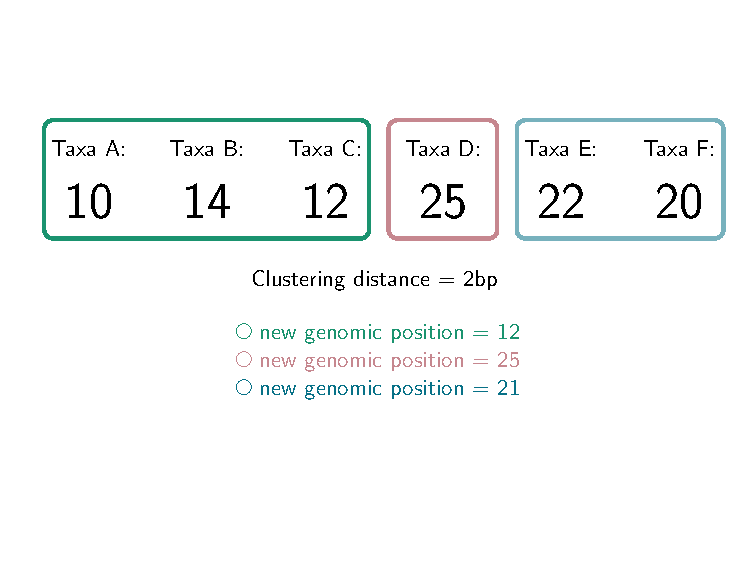
\includegraphics[viewport={\xL} {\yL} {\xR} {\yR},clip,scale=\SecondScale]{./figs/genomic_position_clustering_example_fig.pdf}
		
		\caption{\label{fig:genomic_pos_clustering_ex} Visualization of the genomic position clustering method. In this example, the user specified the genetic distance to be 2, all genomic positions within 2 base pairs would be clustered together. In this example we are looking at 6 taxa with genomic positions 10, 14, 12, 25, 22, and 20. Based on the clustering algorithm, positions 10, 14 and 12 would be grouped into a cluster (outlined in green), position 25 would be its own cluster (outlined in pink), and positions 22 and 20 would be grouped into another cluster (outlined in blue). Once the clusters are determined, a new genomic position for each of the clusters is calculated using the average of all positions within that cluster. In this example, the green cluster would have a new genomic position of 12 (the average between those three positions), the pink cluster would have the sane genomic position of 25, and the blue cluster would have a new genomic position of 21. The new list of genomic positions for the 4 taxa would be: 12, 12, 12, 25, 21 and 21.}
	\end{center}
\end{figure}

		
\begin{table}[H]
	\centering
	\resizebox{\textwidth}{!}{%
		\begin{tabular}{lcccccc}
			\toprule
			Position Difference & \ecol Chromosome &\bass Chromosome & \strep Chromosome & \smel Chromosome &\smel pSymA & \smel pSymB\\
	\midrule
	1bp & -1.394\e{-7}** & -2.538\e{-8}** & 1.736\e{-8}** & -1.541\e{-6}** & -9.130\e{-7}** & 2.488\e{-7}*** \\
	10bp & -1.394\e{-7}*** & -2.518\e{-8}*** & -4.484\e{-9}*** & -1.627\e{-6}*** & -9.13\e{-7}*** & 3.487\e{-7}***\\
	100bp & -1.764\e{-7}*** & -1.417\e{-8}*** & 1.448\e{-8}*** & -1.605\e{-6}*** & -1.166\e{-6}*** & 4.021\e{-7}*** \\
	1000bp & -1.784\e{-7}*** & -1.417\e{-8}*** & 1.505\e{-8}*** & -1.605\e{-6}*** & -1.153\e{-6}*** & 4.021\e{-7}***\\
	10000bp & -1.712\e{-7}*** & -3.496\e{-8}*** & 4.790\e{-8}*** & -1.605\e{-6}*** & -3.570\e{-8}* & 3.784\e{-7}*** \\
	100000bp & -2.061\e{-7}*** & -3.561\e{-8}*** & 4.167\e{-9}*** & -1.605\e{-6}*** & -4.676\e{-7}*** & 3.784\e{-7}***\\
	1000000bp & 4.229\e{-8}*** & -7.710\e{-9}*** & 6.083\e{-8}*** &-1.605\e{-6}*** & 4.285\e{-6}*** & -8.888\e{-7}*** \\
	\bottomrule
		\end{tabular}
		
	}%resizebox
	\caption{\label{tab:clustering} Results from the position clustering analysis. Logistic regression analysis of the number of substitutions along the genome of the respective bacteria replicons to test position differences. The ``Position Difference'' column denotes different base pair distances that the positions in the genome were clustered together as. All results are marked with significance codes as followed: $<$ 0.001 = `***', 0.001 $<$ 0.01 = `**', 0.01 $<$ 0.05 = `*', 0.05 $<$ 0.1 = `.', $>$ 0.1 = ` '. Logistic regression was calculated after the positions in the genome were determined to be the same at each position difference listed in the first column.}
\end{table}	
		
\begin{table}[h]
	\centering
	\resizebox{\textwidth}{!}{%
		\begin{tabular}{lrrr}
			\toprule
			Bacteria and Replicon & Average Replicon Length  & Number of Sites & Number of Substitutions \\
			\midrule
			\ecol Chromosome & 5082529 & 2318259 & 353740 \\ % 4048616/4641652 & 
			\bass Chromosome & 4077077 & 2032176 & 185060 \\ %3692179/4215606
			\strep Chromosome & 8494093 & 6057063 & 24046  \\ % 7628849/8667507
			\smel Chromosome & 3426881 & 1892874 & 11210\\ % 3130925/3654135
			\smel pSymA & 1455940 & 571278 & 13132 \\ % 1128615/1354226 & 225611/1354226
			\smel pSymB & 1664597 & 1248879  & 28941 \\ % 1493048/1683333
			\bottomrule
		\end{tabular}
		
	}%resizebox
	\caption{\label{tab:cod_non_cod_proportions} Total number of protein coding sites in each replicon for this analysis and the number of those sites that have a substitution (multiple substitutions at one site are counted as two substitutions).}
\end{table}

\newpage
%%%%%%%%%%%%%%%%%%%%%%%%%%%%%%%%%%%%%%%%%%%%%%%%%%%%%%%%%%%%%%%%%%%%%%%%%%%%
\subsection{High Substitutions Gene Example}
Throughout this analysis there are a few genes/gene segments in all the bacterial replicons that have relatively high numbers of substitutions when compared to other genes or gene segments.
These high numbers of substitutions are indeed real changes seen in homologous genes.
To illustrate this, we have chosen a segment of alignment from \strep.
Information about the genes involved in this segment can be found in Table \ref{tab:high_subs_gene_info}.
A protein alignment for these genes can be found on \texttt{GitHub} (\url{https://github.com/dlato/Spatial_Patterns_of_Substitutions}) under the file name ``\texttt{Streptomyces\_high\_substitutions\_gene\_example.txt}''.

Both \sliv strains have 100\% sequence identity at the DNA level, while the \scoe species has 87.2\% sequence identity with the \sliv strains for this particular alignment.
Dispite this high sequence identity and almost identical protein alignment (Figures \ref{fig:nucaln} and \ref{fig:protaln}), there are a total of 31 substitutions (across all nodes of the phylogenetic tree, Figure \ref{fig:streptree}) within this short stretch of sequence.
It is segments like these that are resulting in the appearance of extremely high numbers of substitutions in sections of all the bacterial repliconic genomes.

\begin{table}[h]
	\centering
	\resizebox{\textwidth}{!}{%
		\begin{tabular}{lcc}
			\toprule
			Species & NCBI Acession Number  & Gene Id \\
			\midrule
			\scoe A3 & AL645882 & SCO6334 \\
			\sliv 1362 & NZ\_CM001889  & SLI\_RS32020  \\
			\sliv TK24 & NZ\_GG657756 & SSPG\_RS06405 \\
			\bottomrule
		\end{tabular}
		
	}%resizebox
	\caption{\label{tab:high_subs_gene_info} Information about the example gene segment with high number of substitutions.}
	%block5_0368_0011_0000
\end{table}

	\begin{figure}[H]
	\begin{center}
		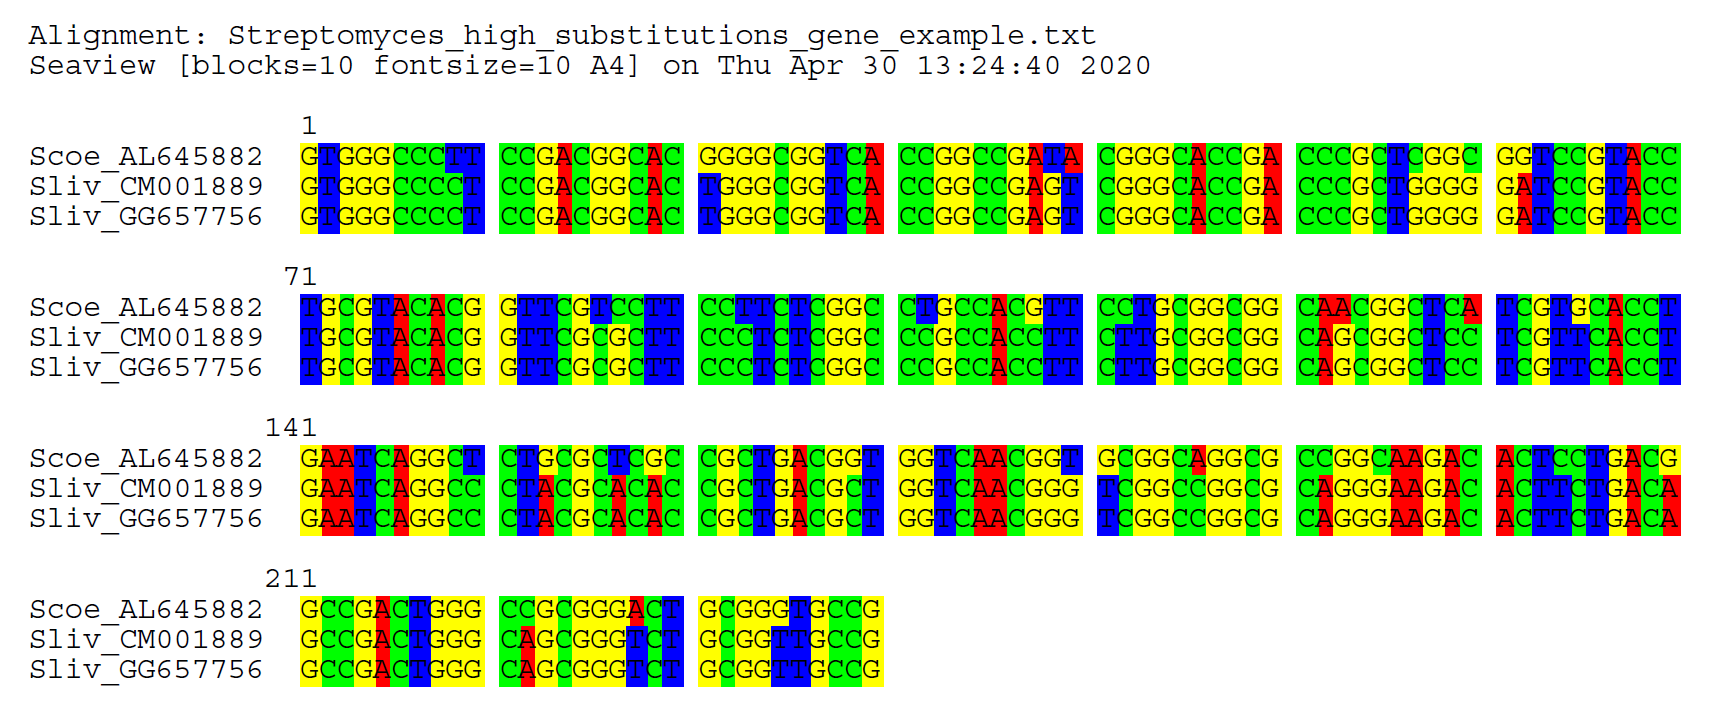
\includegraphics[width=\textwidth]{./figs/Streptomyces_high_substitutions_gene_example_nucleotide_alnment.png}
		\caption{\label{fig:nucaln} Visualization of the nucleotide alignment of \strep genes with high numbers of substitutions. Alignment visualization was performed with \texttt{SeaView} \citep{Gouy:10}}
	\end{center}
\end{figure}


	\begin{figure}[H]
	\begin{center}
		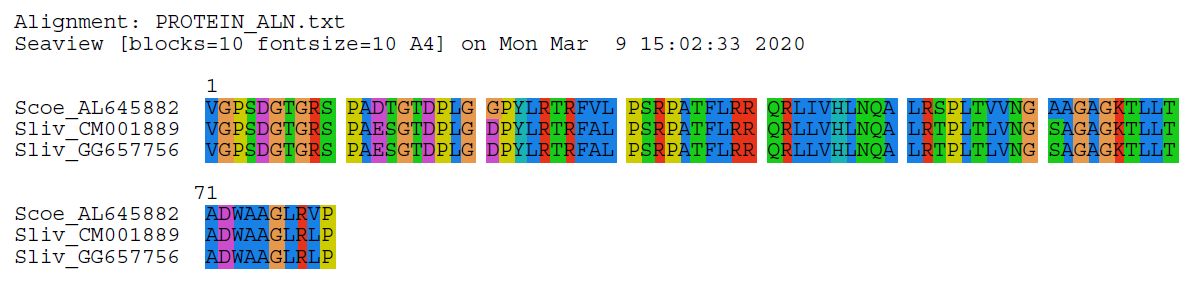
\includegraphics[width=\textwidth]{./figs/Streptomyces_high_substitutions_gene_example.png}
		\caption{\label{fig:protaln} Visualization of the protein alignment of \strep genes with high numbers of substitutions. Alignment visualization was performed with \texttt{SeaView} \citep{Gouy:10}}
	\end{center}
\end{figure}




\subsection{High Substitution Distribution}
\begin{longtable}{lcl}
	\hline
	Bacteria and Replicon & Bidirectional Genomic Position (bp) & Protein/Gene Examples \\ \hline
	\ecol Chromosome & 1130000 - 1140000 & Uncharacterized protein\\
	& & Hypothetical protein\\
	& & Lipoprotein\\ 
	& & Transcriptional activator\\ 
	& 1720000 - 1740000 & Hypothetical protein\\
	& & Predicted protein\\
	& & Small toxic polypeptide\\ \hline
	\bass Chromosome & 560000 - 570000 & Hypothetical protein\\
	& & Derived by automated\\
	& & computational analysis\\
	& & Membrane protein\\
	& 1820000 - 1380000 & Derived by automated\\
	& & computational analysis\\ \hline
	\strep Chromosome & 3550000 - 3570000 & Hypothetical protein\\
	& & Derived by automated\\
	&  & computational analysis\\
	& & Putative integral membrane protein\\
	& & Reductase \\ \hline
	\smel Chromosome & 80000 - 90000 & Hypothetical proteins\\
	&  730000 - 740000 & Hypothetical proteins\\
	& & Putative proteins\\\hline
	\smel \pa & 100000 - 110000 & Hypothetical proteins\\
	& 800000 - 810000 & Hypothetical protein \\
	& & Transporter protein \\ \hline
	\smel \pb & 450000 - 460000 & Hypothetical protein\\
	& & Putative oxidoreductase\\
	& & Hypothetical proteins\\
	& 610000 - 620000 & Hypothetical protein\\
	& & Putative transport regulator\\
	& & Predicted membrane protein\\ \hline
	%	& 800000 - 810000 & Small molecule metabolism\\
	\caption{\label{tab:high_sub_bars} Table of high number of substitutions per 10Kbp genomic regions for each bacterial replicon and examples of the associated proteins/gene functions found in that region. The genomic position begins at the origin of replication and continues in both directions until the terminus of replication (bidirectional replication).}
\end{longtable}

%%%%%%%%%%%%%%%%%%%%%%%%%%%%%%%%%%%%%%%%%%%%%%%%%%%%%%%%%%%%%%%%%%%%%%%%%%%%%%%%
\subsection{Weighted, Non-weighted, and 20Kbp Near and Far From the Origin Substitution Linear Regression Analysis}
\begin{table}[h]
	\centering
	\resizebox{\textwidth}{!}{%
		\begin{tabular}{lcccccc}
		\toprule
		& \multicolumn{6}{c}{Protein Coding Window Size}  \\
		\cmidrule{2-7}
		Bacteria and Replicon & 10Kbp & 25Kbp & 50Kbp & 100Kbp & 200Kbp & 400Kbp \\
		%			& Coefficient Estimate & $R^2$ & Coefficient Estimate & $R^2$ \\
		\midrule
		\ecol Chromosome & -1.66\e{-4}***& -4.18\e{-4}***  & -8.64\e{-4}*** & -1.71\e{-3}*** & -3.42\e{-3}** & -6.71\e{-3}*\\
		& (0.398)& (0.476) & (0.563) & (0.509) & (0.534) & (0.592)\\
		\midrule
		%%%%%%%%%%%%%%%%%%%%%%%%%%%%%%%%%%%%%%%%%%%%%%%%%%%
		\bass Chromosome & NS & NS & NS & NS & NS & NS \\
		& (0.009) & (0.001) & (0.0002) & (0.002) & (0.019) & (0.484)\\
		\midrule
		%%%%%%%%%%%%%%%%%%%%%%%%%%%%%%%%%%%%%%%%%%%%%%%%%%%
		\strep Chromosome &  -6.78\e{-7}*& NS & NS & NS & NS & NS\\
		& (0.005) & (0.006) & (0.010) & (0.027) & (0.083) & (0.091)\\
		\midrule
		%%%%%%%%%%%%%%%%%%%%%%%%%%%%%%%%%%%%%%%%%%%%%%%%%%%
		\smel Chromosome &  -8.97\e{-6}**& -3.72\e{-5}** & -7.76\e{-5}* &-1.64\e{-4}* & NS & NS\\
		& (0.040) & (0.098) & (0.126) & (0.188) & (0.082) & (0.427)\\
		\midrule
		%%%%%%%%%%%%%%%%%%%%%%%%%%%%%%%%%%%%%%%%%%%%%%%%%%%
		\smel \pa & NS& NS & NS & NS & NS & NS\\
		& (0.032) & (0019) & (0.135) &(0.0124) & (0.034) & (1.42\e{-30})\\
		\midrule
		%%%%%%%%%%%%%%%%%%%%%%%%%%%%%%%%%%%%%%%%%%%%%%%%%%%
		\smel \pb &  NS & NS & NS &NS & NS & NS\\
		& (0.001) & (0.003) & (0.008) & (0.006) & (2.12\e{-8}) & (0.043)\\
		\bottomrule
		
		\end{tabular}
		
	}%resizebox
	\caption{\label{tab:lin_reg_windows_subs_weighted} Linear regression on various sections of the genome (10Kbp, 25Kbp, 50Kbp, 100Kbp, 200Kbp, and 400Kbp) with increasing distance from the origin of replication after accounting for bidirectional replication. The total number of substitutions in each section of the genome was divided by the total number of protein coding sites in that genomic region. All results are marked with significance codes as followed: $<$ 0.001 = `***', 0.001 $<$ 0.01 = `**', 0.01 $<$ 0.05 = `*', $>$ 0.05 = `NS'. The $R^2$ value for each coefficient estimate is found below the value in brackets ().}
\end{table}



\begin{table}[h]
	\centering
	\resizebox{\textwidth}{!}{%
	\begin{tabular}{lcccccc}
		\toprule
		& \multicolumn{6}{c}{Protein Coding Window Size}  \\
		\cmidrule{2-7}
		Bacteria and Replicon & 10Kbp & 25Kbp & 50Kbp & 100Kbp & 200Kbp & 400Kbp \\
		%			& Coefficient Estimate & $R^2$ & Coefficient Estimate & $R^2$ \\
		\midrule
		\ecol Chromosome & -2.27\e{-9}*** & -2.54\e{-10}** & -2.32\e{-10}* & -2.36\e{-10}*** & NS & NS\\
		& (0.039)& (0.078) & (0.112) & (0.133) & (0.200) & (0.361)\\
		\midrule
		%%%%%%%%%%%%%%%%%%%%%%%%%%%%%%%%%%%%%%%%%%%%%%%%%%%
		\bass Chromosome & NS & NS & NS & NS & NS & NS\\
		& (0.004) & (0.004) & (0.001) & (0.001) & (0.145) & (0.027)\\
		\midrule
		%%%%%%%%%%%%%%%%%%%%%%%%%%%%%%%%%%%%%%%%%%%%%%%%%%%
		\strep Chromosome &  NS & NS & NS & 2.69\e{-11}* & 4.09\e{-11}** & NS\\
		& (5\e{-5})& (3\e{-8}) & (0.004) & (0.064) & (0.248) & (0.060)\\
		\midrule
		%%%%%%%%%%%%%%%%%%%%%%%%%%%%%%%%%%%%%%%%%%%%%%%%%%%
		\smel Chromosome &  -1.21\e{-10}*** & -1.71\e{-10}*** & -1.86\e{-10}** & -2.78\e{-10}** & NS & NS\\
		& (0.076) & (0.137) & (0.253) &(0.350) & (0.150) & (0.397)\\
		\midrule
		%%%%%%%%%%%%%%%%%%%%%%%%%%%%%%%%%%%%%%%%%%%%%%%%%%%
		\smel \pa &  NS & NS & NS & NS & NS & NS\\
		& (0.027) & (0.001) & (0.006) & (0.193) & (0.050) & (1.59\e{-31})\\
		\midrule
		%%%%%%%%%%%%%%%%%%%%%%%%%%%%%%%%%%%%%%%%%%%%%%%%%%%
		\smel \pb &  NS & NS & NS & NS & NS & NS\\
		& (0.035) & (0.053) & (0.010) & (0.002) & (0.495) & (0.491)\\
		\bottomrule
		\end{tabular}
		
	}%resizebox
	\caption{\label{tab:lin_reg_windows_subs_nonweighted} Linear regression on various sections of the genome (10Kbp, 25Kbp, 50Kbp, 100Kbp, 200Kbp, and 400Kbp) with increasing distance from the origin of replication after accounting for bidirectional replication. The linear regression was performed on the total number of substitutions in each section of the genome without accounting for the number of sites in each genomic region. All results are marked with significance codes as followed: $<$ 0.001 = `***', 0.001 $<$ 0.01 = `**', 0.01 $<$ 0.05 = `*', $>$ 0.05 = `NS'. The $R^2$ value for each coefficient estimate is found below the value in brackets ().}
\end{table}




\begin{table}[h]
	\centering
	\resizebox{\textwidth}{!}{%
		\begin{tabular}{lcc|cc}
			\toprule
			& \multicolumn{4}{c}{Protein Coding} \\
			\cmidrule{2-5}
			%			\cmidrule{8-10}
			%			& \multicolumn{3}{c}{Weighted} & \multicolumn{3}{c}{Non-weighted} & \multicolumn{3}{c}{Weighted} \\
			%			\cmidrule{2-3}
			%			\cmidrule{4-7}
			& \multicolumn{2}{c|}{Correlation Coefficient} & \multicolumn{2}{c}{Number of Substitutions} \\
			& \multicolumn{2}{c|}{20kb Near} &\multicolumn{2}{c}{per 20kb Near}\\
			\cmidrule{2-5}
			Bacteria and Replicon &  Origin & Terminus& Origin & Terminus\\
			\midrule
			\ecol Chromosome & 6.51\e{-6}** & 6.16\e{-6}** & 5.85\e{-3} & 6.47\e{-3} \\
			\bass Chromosome & 1.18\e{-6}* & 1.57\e{-5}*** & 4.23\e{-3} & 5.01\e{-3} \\
			\strep Chromosome & NS & NS & 4.11\e{-4} & 2.05\e{-5} \\
			\smel Chromosome & 7.11\e{-6}*** & NS & 1.51\e{-3}  & 3.86\e{-5}\\
			\smel pSymA & -6.94\e{-5}***  & NS & 2.03\e{-3} & 3.27\e{-3}\\
			\smel pSymB & 1.58\e{-5}*** & -7.10\e{-5}*** & 3.06\e{-3} &  1.25\e{-3} \\
			\bottomrule
		\end{tabular}
		
	}%resizebox
	\caption{\label{tab:20kb_near_far_ori} Logistic regression on 20kb closest and farthest from the origin of replication after accounting for bidirectional replication and outliers. Number of substitutions was calculated by taking the total number of substitutions in each of the 20Kbp regions and dividing by the total number of sites in those regions. All results are marked with significance codes as followed: $<$ 0.001 = `***', 0.001 $<$ 0.01 = `**', 0.01 $<$ 0.05 = `*', $>$ 0.05 = `NS'. The $R^2$ values for each estimate are in brackets.}
\end{table}

Multiple linear regressions were performed to determine if there was any correlation between number of substitutions and distance from the origin of replication.
A linear regression to determine how the weighted and non-weighted total number of substitutions in various sections of the genome (10Kbp, 25Kbp, 50Kbp, 100Kbp, 200Kbp, and 400Kbp) changes with genomic position was performed  (Tables \ref{tab:lin_reg_windows_subs_weighted} and \ref{tab:lin_reg_windows_subs_nonweighted}).
All additional linear regression results (Tables \ref{tab:lin_reg_windows_subs_weighted} and \ref{tab:lin_reg_windows_subs_nonweighted}) mirror the results from the logistic regression on presence or absence of substitutions and changes in genomic position (see the Main Paper results section for more information).
The results from these supplemental tests are consistent with the results from the linear regression found in the Main Paper, most bacterial replicons have a decreasing number of substitutions when moving away from the origin of replication.

To calculate the non-weighted values of the total number of substitutions per 10Kbp region of the genome, the total number of substitutions was summed up over each region of the genome (10Kbp, 25Kbp, 50Kbp, 100Kbp, 200Kbp, and 400Kbp), while accounting for bidirectional replication (see Main Paper for details).
A linear regression on these total number of substitutions in each section of the genome (10Kbp, 25Kbp, 50Kbp, 100Kbp, 200Kbp, and 400Kbp) was performed to see how the number of substitutions changes with distance from the origin of replication (Table \ref{tab:lin_reg_windows_subs_nonweighted}).
The weighted values of the total number of substitutions per various region of the genome, the total number of substitutions was summed up over each region of the genome (10Kbp, 25Kbp, 50Kbp, 100Kbp, 200Kbp, and 400Kbp) while accounting for bidirectional replication (see Main Paper for details).
These summed values were then divided by the total number of protein coding sites in each region to obtain the weighted value.
A linear regression on these weighted total number of substitutions in each section of the genome was performed to see how the number of substitutions changes with distance from the origin of replication (Table \ref{tab:lin_reg_windows_subs_weighted}).

We took a closer look at 20Kbp regions of the replicons close and far from the origin of replication.
We performed a logistic regression on the presence or absence of a substitution with distance from the origin of replication.
Data points from the 20Kbp regions closest to the origin of replication and data points from the 20Kbp regions closest to the terminus of replication were used for this portion of the analysis.
Outliers were removed from this analysis.
The number of substitutions per site was also calculated in each of these 20Kbp regions for each bacterial replicon.
We were unable to determine a consistent spatial substitution trend when considering only the 20Kbp near and far from the orign of replication in all bacterial replicons.
Some bacterial replicons had a positive correlation coefficient, indicating that the number of substitutions increases with increasing distance from the origin of replication (Table \ref{tab:20kb_near_far_ori}).
Other replicons had a negative correlation coefficient, suggesting that the number of substitutions decreases with increasing distance from the origin of replication (Table \ref{tab:20kb_near_far_ori}).
Additionally, it was unclear if the number of substitutions per site locally were higher near the origin of replication or near the terminus.
Some bacteria had higher number of substitutions per site near the origin (\ecol, \smel chromosome and \pb), while other replicons has the opposite trend (\bass, \strep and \smel \pa) (Table \ref{tab:20kb_near_far_ori}).
These results suggest that on a small local scale, there are varying patterns of substitutions with respect to distance from the origin of replication.
This varies between bacteria, and in some cases even within the same bacteria (\ecol).
This variation locally does not allow us to make any overarching statements about the local distribution of substitutions in bacterial genomes.
It is therefore more useful to consider the global (genome wide) pattern of substitutions when making overarching statements about genomic substitution arrangements.


\subsection{Non-linear Analysis of Number of Substitutions and Distance From the Origin of Replication}

Using a simple smoothed conditional means method (\texttt{geom\_smooth()} function in \texttt{R}), a non-linear trend analysis was performed on all bacterial replicons.
The previous mentioned weighted data (see the previous subsection), was used in this analysis.
The weighted data represents the total number of substitutions divided by the total number of protein-coding sites in 10Kbp segments of the genomes.
Outliers were removed.
The results from this non-linear analysis can be seen in Figures \ref{fig:ecoli_nonpar} - \ref{fig:pSymB_nonpar}.
The visual results from this analysis mirror the findings from the main paper, the total number of substitutions varies with distance from the origin of replication, but the direction of this trend is unclear and inconsistent between bacterial replicons.
 



\begin{figure}[h]
	\begin{center}
		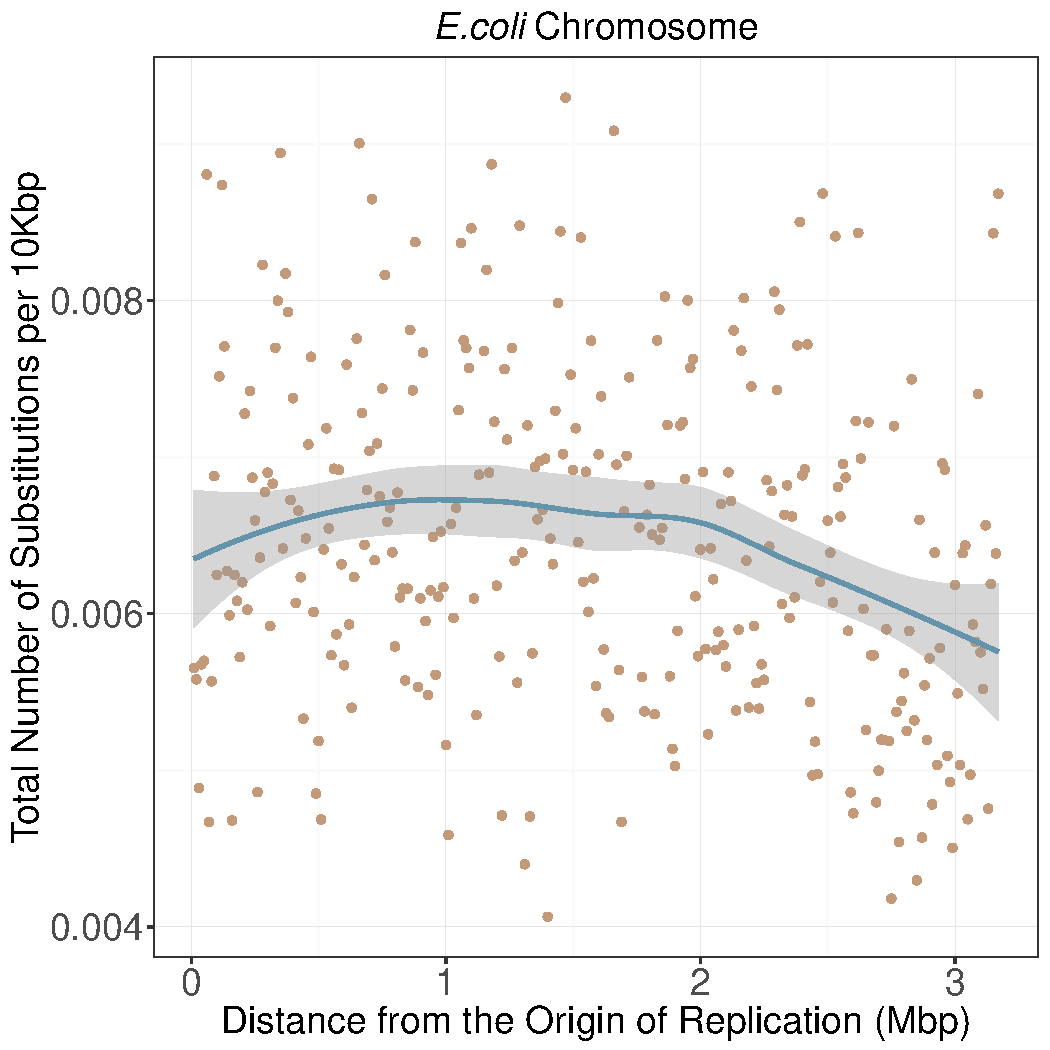
\includegraphics[width=\textwidth]{./figs/ecoli_10KB_weighted_subs_nonpar_12Sep20.pdf}
		\caption{\label{fig:ecoli_nonpar}The graph shows the total number of substitutions weighted by the total number of protein-coding sites per 10Kbp segments of the \ecol genome. Each of these individual values are represented by beige coloured circles. A non-linear trend line (using the \texttt{geom\_smooth()} function in \texttt{R}), was fit to these average values and the associated 95\% confidence intervals for this line is represented by the grey ribbon around the blue trend line. Outliers were removed from this graph.}
	\end{center}
\end{figure}

\begin{figure}[h]
	\begin{center}
		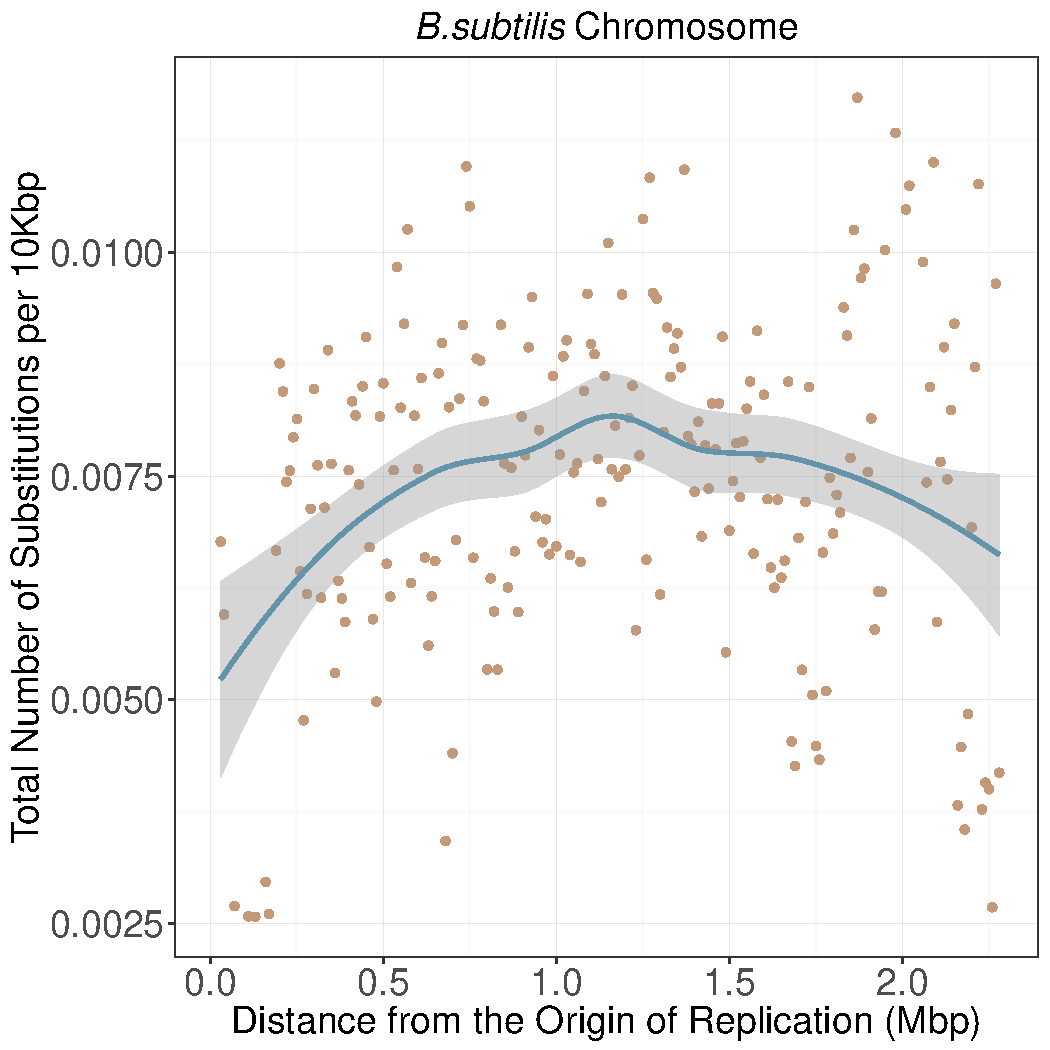
\includegraphics[width=\textwidth]{./figs/bass_10KB_weighted_subs_nonpar_22Sep20.pdf}
		\caption{\label{fig:bass_nonpar}The graph shows the total number of substitutions weighted by the total number of protein-coding sites per 10Kbp segments of the \bass genome. Each of these individual values are represented by beige coloured circles. A non-linear trend line (using the \texttt{geom\_smooth()} function in \texttt{R}), was fit to these average values and the associated 95\% confidence intervals for this line is represented by the grey ribbon around the blue trend line. Outliers were removed from this graph.}
	\end{center}
\end{figure}

\begin{figure}[h]
	\begin{center}
		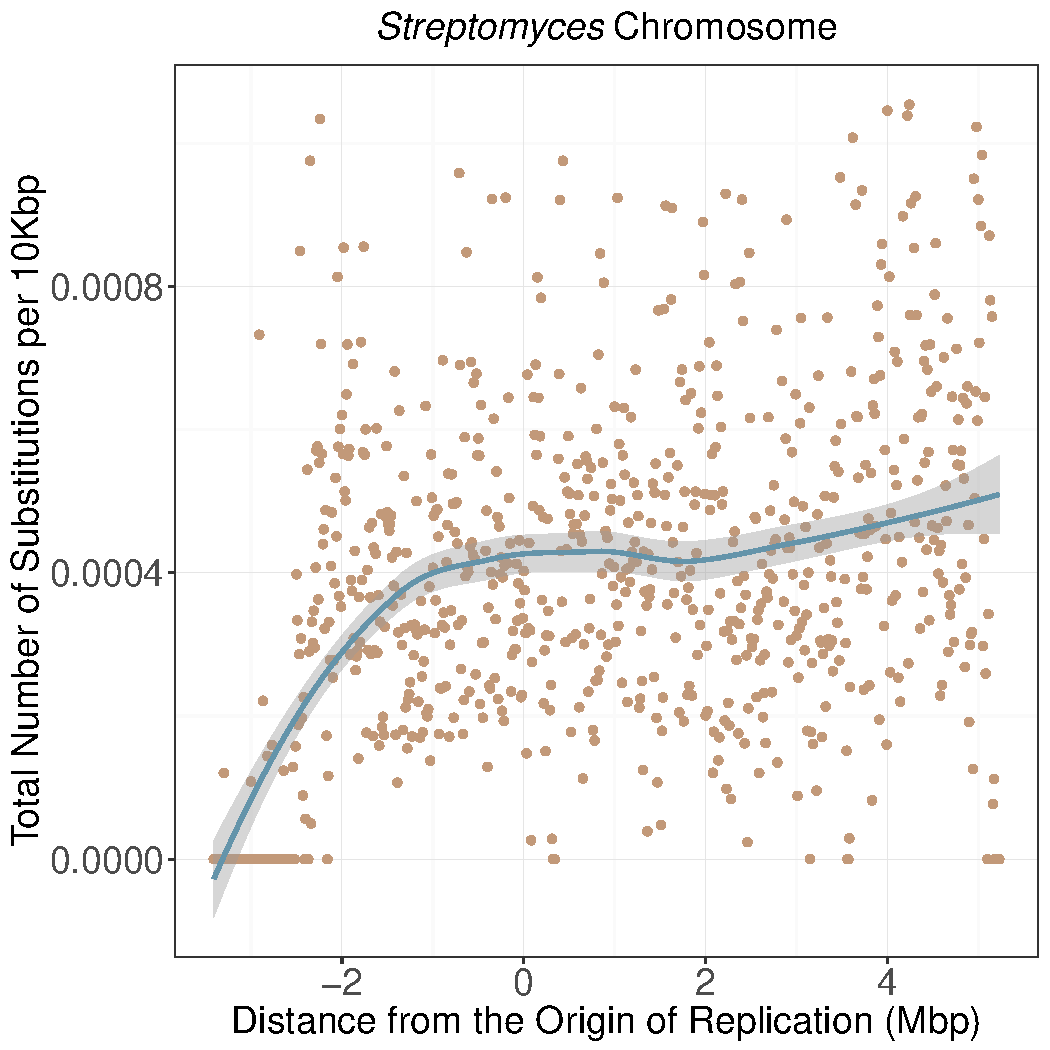
\includegraphics[width=\textwidth]{./figs/strep_10KB_weighted_subs_nonpar_14Sep20.pdf}
		\caption{\label{fig:strep_nonpar}The graph shows the total number of substitutions weighted by the total number of protein-coding sites per 10Kbp segments of the \strep genome. Each of these individual values are represented by beige coloured circles. A non-linear trend line (using the \texttt{geom\_smooth()} function in \texttt{R}), was fit to these average values and the associated 95\% confidence intervals for this line is represented by the grey ribbon around the blue trend line. Outliers were removed from this graph.}
	\end{center}
\end{figure}


\begin{figure}[h]
	\begin{center}
		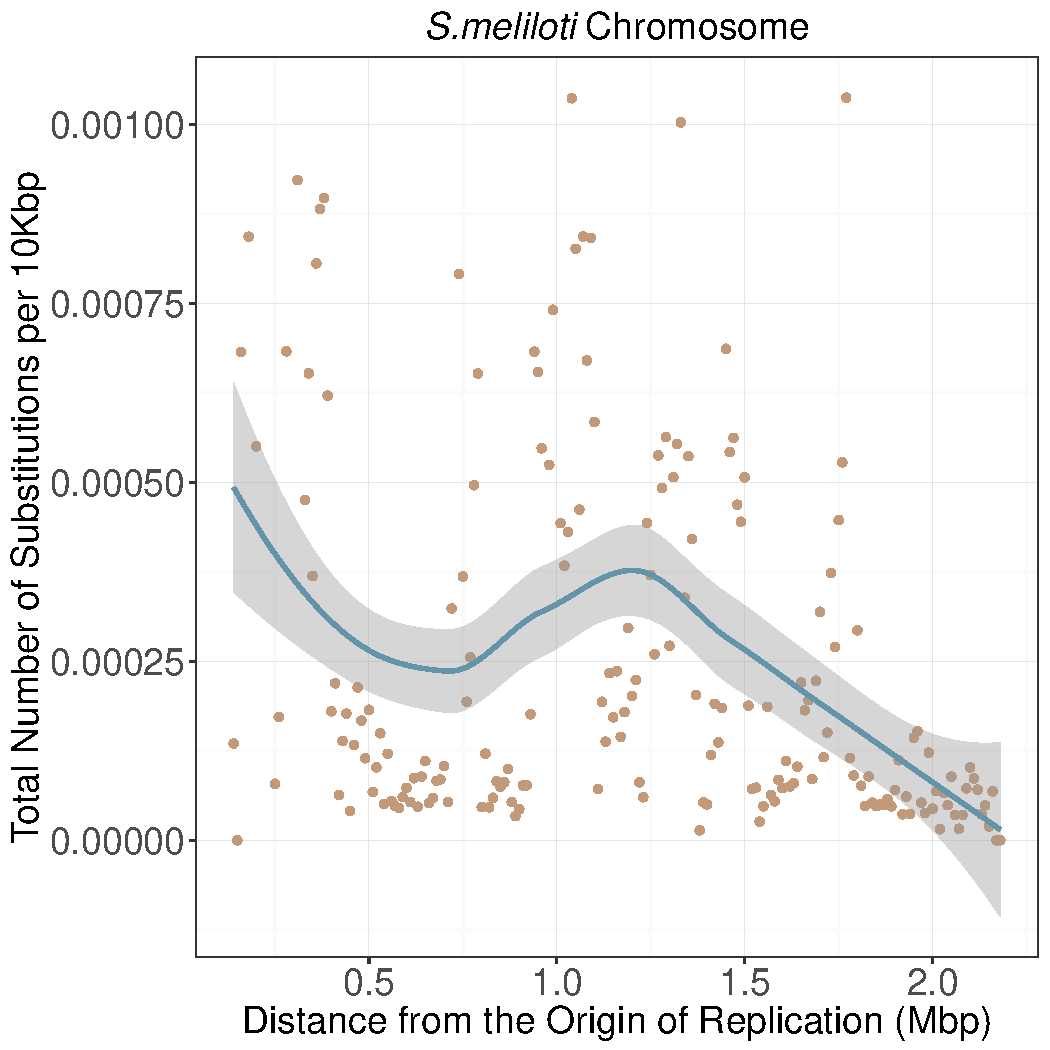
\includegraphics[width=\textwidth]{./figs/sinoC_10KB_weighted_subs_nonpar_12Sep20.pdf}
		\caption{\label{fig:sinoC_nonpar}The graph shows the total number of substitutions weighted by the total number of protein-coding sites per 10Kbp segments of the \smel Chromosome. Each of these individual values are represented by beige coloured circles. A non-linear trend line (using the \texttt{geom\_smooth()} function in \texttt{R}), was fit to these average values and the associated 95\% confidence intervals for this line is represented by the grey ribbon around the blue trend line. Outliers were removed from this graph.}
	\end{center}
\end{figure}

\begin{figure}[h]
	\begin{center}
		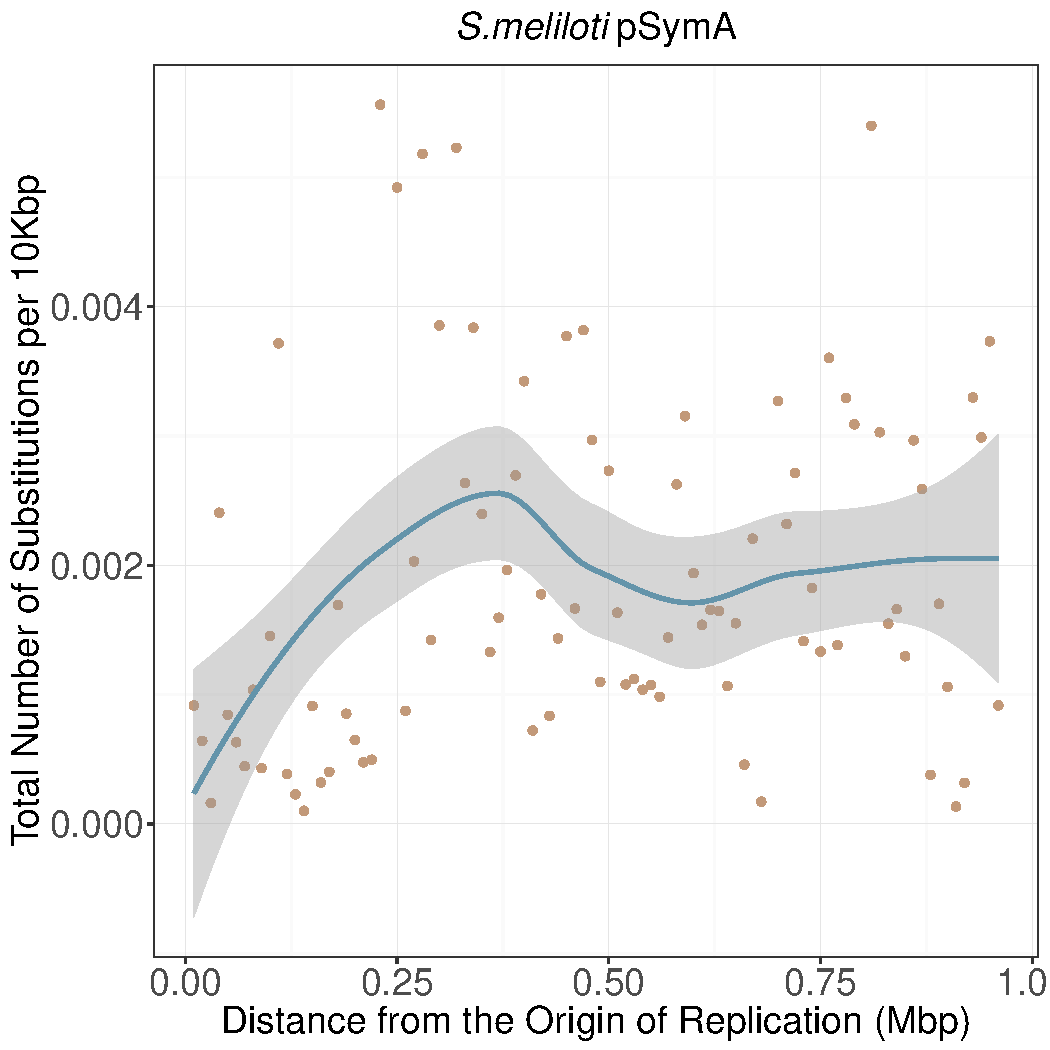
\includegraphics[width=\textwidth]{./figs/pSymA_10KB_weighted_subs_nonpar_22Sep20.pdf}
		\caption{\label{fig:pSymA_nonpar}The graph shows the total number of substitutions weighted by the total number of protein-coding sites per 10Kbp segments of the \smel \pa replicon. Each of these individual values are represented by beige coloured circles. A non-linear trend line (using the \texttt{geom\_smooth()} function in \texttt{R}), was fit to these average values and the associated 95\% confidence intervals for this line is represented by the grey ribbon around the blue trend line. Outliers were removed from this graph.}
	\end{center}
\end{figure}

\begin{figure}[h]
	\begin{center}
		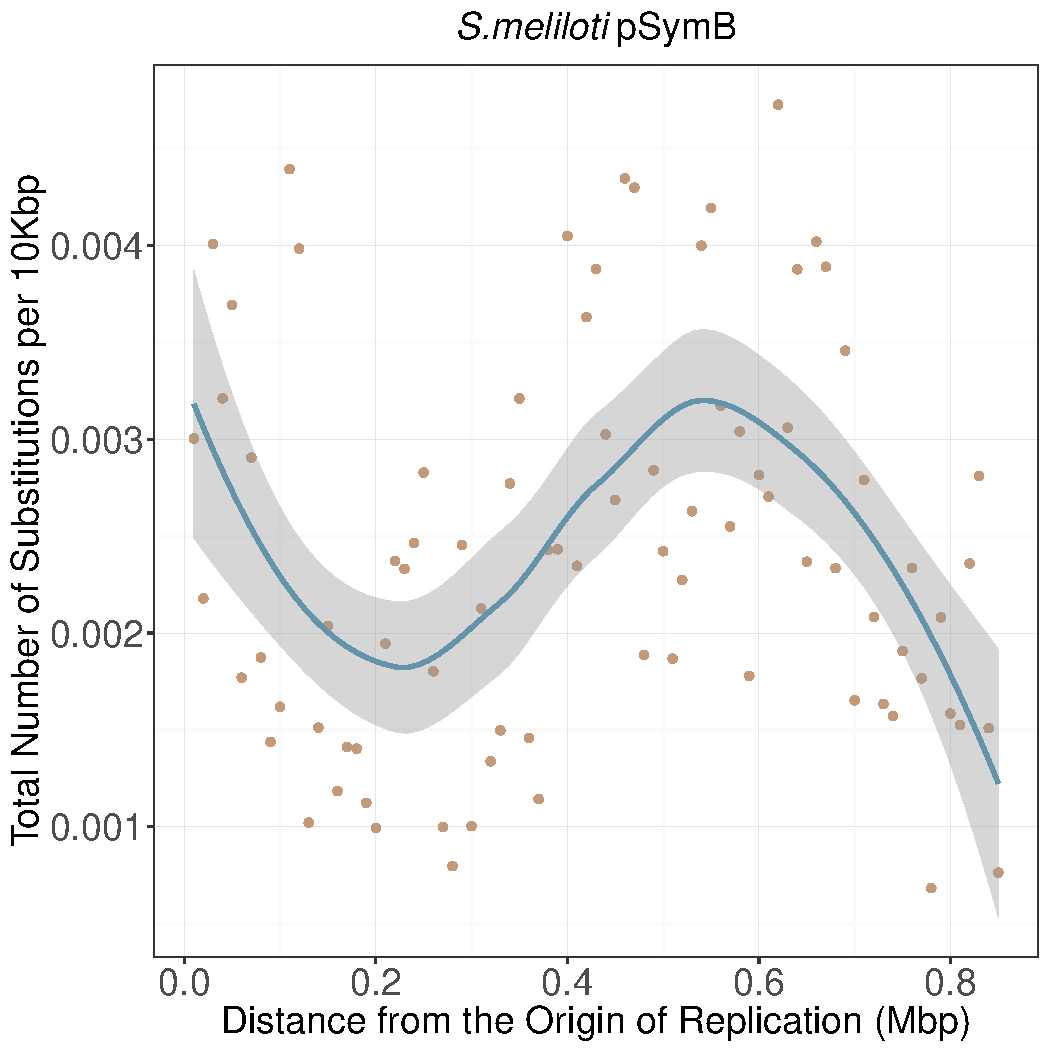
\includegraphics[width=\textwidth]{./figs/pSymB_10KB_weighted_subs_nonpar_22Sep20.pdf}
		\caption{\label{fig:pSymB_nonpar}The graph shows the total number of substitutions weighted by the total number of protein-coding sites per 10Kbp segments of the \smel \pb replicon. Each of these individual values are represented by beige coloured circles. A non-linear trend line (using the \texttt{geom\_smooth()} function in \texttt{R}), was fit to these average values and the associated 95\% confidence intervals for this line is represented by the grey ribbon around the blue trend line. Outliers were removed from this graph.}
	\end{center}
\end{figure}

\subsection{Total Number of Sites Linear Regression}

We performed a linear regression on the total number of protein coding sites and distance from the origin of replication.
We found that the total number protein coding sites decreases with distance from the origin of replication in majority of the bacterial replicons in this analysis.
We were unable to detect a significant relationship between the number of protein coding sites and distance from the origin of replication in \pb of \smel.


\begin{table}[h]
	\centering
	\resizebox{0.75\textwidth}{!}{%
		\begin{tabular}{lcc}
			\toprule
			Bacteria and Replicon & Coefficient Estimate & $R^2$\\
			\midrule
			\ecol Chromosome & -2.33\e{-2}*** & 0.423\\
			\bass Chromosome & NS & 0.001\\
			\strep Chromosome & -1.24\e{-3}*** & 0.069\\
			\smel Chromosome & NS & 0.096\\
			\smel pSymA & NS  & 0.002\\
			\smel pSymB & 2.69\e{-2}** & 0.081\\
			\bottomrule
		\end{tabular}
		
	}%resizebox
	\caption{\label{tab:lr_gene_num} Linear regression analysis of the total number of protein coding sites per 10kb along the genome of the respective bacteria replicons. Linear regression was calculated after the origin of replication was moved to the beginning of the genome and all subsequent positions were scaled around the origin accounting for bidirectionality of replication. All results are marked with significance codes as followed: $<$ 0.001 = `***', 0.001 $<$ 0.01 = `**', 0.01 $<$ 0.05 = `*', $>$ 0.05 = `NS'.}
\end{table}

%%%%%%%%%%%%%%%%%%%%%%%%%%%%%%%%%%%%%%%%%%%%%%%%%%%%%%%%%%%%%%%%%%%%%%%%%%%%


\newpage
\subsection{Average \dn, \ds, and $\omega$ per Gene Values}
The average \dn, \ds, and $\omega$ values per gene were calculated.
For genes that were split into multiple parts (due to the presence of gaps or poor homology in the alignment), the \dn, \ds, and $\omega$ values for each gene part were averaged to obtain a single average value per gene.
A complete list of these values can be found on \texttt{GitHub} (\url{www.github.com/dlato/Spatial\_Patterns\_of\_Substitutions}) under the file name ``\texttt{Supplementary\_table\_per\_gene\_dN\_dS\_omega.pdf}''.

	\subsection{Distribution of \dn, \ds, and $\omega$}
	\begin{figure}
		\centering
		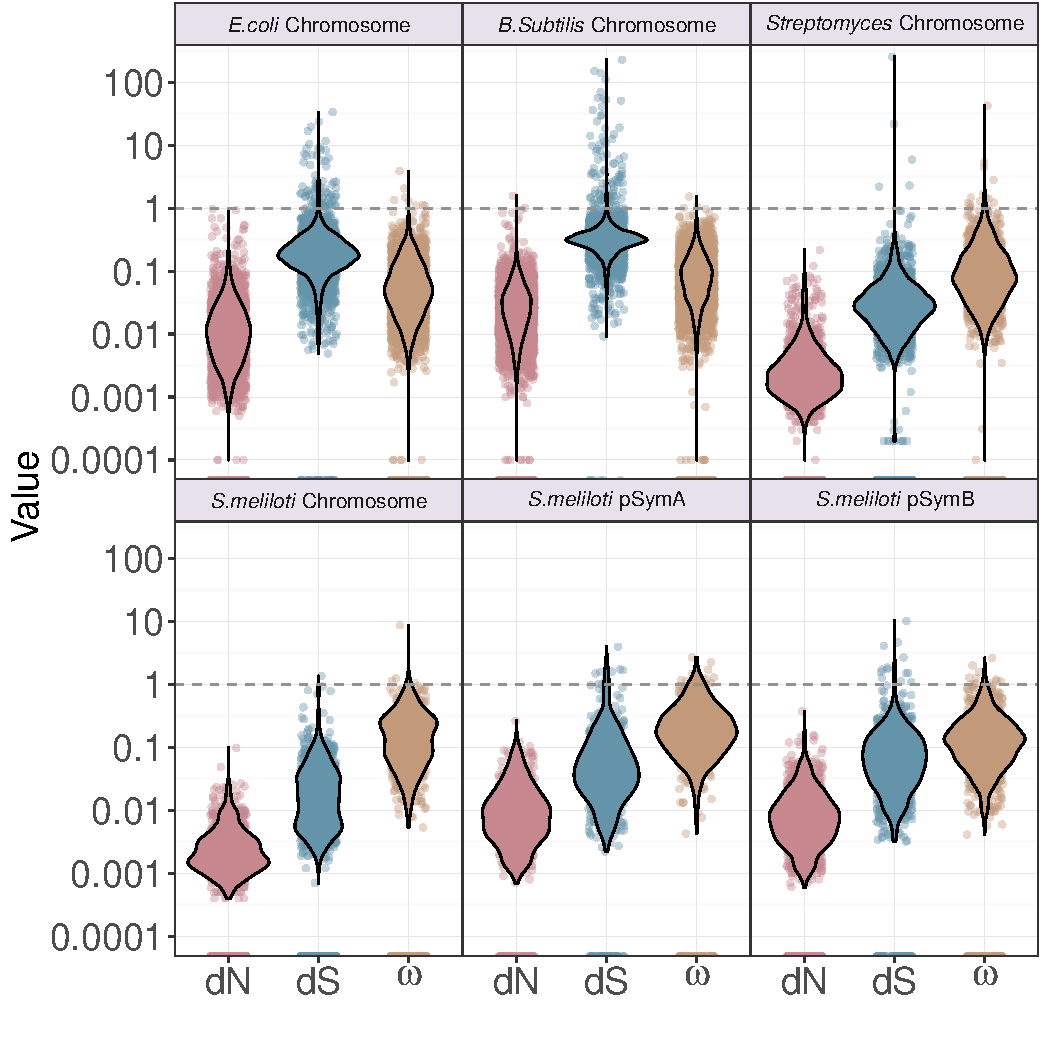
\includegraphics[width=\textwidth]{./figs/ALL_BAC_dN_dS_omega_violinplots_22Sep20.pdf}
		\caption{\label{fig:box_plots} Distribution of all \dn, \ds, and $\omega$ values on a log base 10 scale for each replicon. Individual points are shown as a strip chart (which has been jittered in the x-direction in \texttt{R} \citep{Wickham2019}), and the density of these selection values is shown in the overlaid violin plot. All points are included in this graphic including outliers. For more information on how outliers were calculated, please see the main paper. Any \dn, \ds, or $\omega$ values that had a value of zero is pushed to the bottom of the x-axis. Since these values will not appear on a log base 10 scale, they are not included in the violin portions of this graphic. For a complete list of zero values in each of the selection categories please refer to Table \ref{tab:selection_outliers}. In these graphs there is a horizontal line of values at 0.0001 for most of the selection coefficients in most of the bacterial replicons. This is due to rounding practices when \texttt{codeml} \citep{Yang97} calculates \dn, \ds, and $\omega$ values.}
	\end{figure}



\begin{table}[h]
	\centering
	\resizebox{\textwidth}{!}{%
		\begin{tabular}{lcccc}
			\toprule
			Bacteria and Replicon & Outliers (\%)   &  \multicolumn{3}{c}{Zero Value (\%)}  \\
			&  &\dn & \ds & $\omega$ \\
			\midrule
			\ecol Chromosome & 7.49 & 13.82 & 1.05 & 13.82 \\
			\bass Chromosome & 5.41 & 4.40 & 0.16 & 4.40 \\
			\strep Chromosome & 4.74 & 25.70 & 14.48 & 25.70 \\
			\smel Chromosome & 17.05 & 61.21 & 59.26 & 61.21\\
			\smel pSymA & 6.69 & 11.28 & 9.75 & 11.28 \\
			\smel pSymB & 6.13 & 13.20 & 5.20 & 13.20\\
			\bottomrule
		\end{tabular}
		
	}%resizebox
	\caption{\label{tab:selection_outliers} Percent of data that was calculated to be an outlier or had a selection variable (\dn, \ds, and $\omega$) value of zero.}
\end{table}



%%%%%%%%%%%%%%%%%%%%%%%%%%%%%%%%%%%%%%%%%%%%%%%%%%%%%%%%%%%%%%%%%%%%%%%%%%%%%%%%
\subsection{20Kbp Near and Far From Origin Selection Linear Regression Analysis}
\label{20Kbp_near_far}
We additionally took a closer look at 20 genes close and far from the origin of replication.
We performed a linear regression on the change in selection values (\dn, \ds, and $\omega$) with distance from the origin of replication in these genes (Table \ref{tab:dN_dS_20genes}).
For majority of the bacterial replicons we failed to find a trend, which is not surprising since there was no evidence of an overall genomic trend when looking at these values (see Main Paper for results).
Again, we are unable to conclude that there is a consistent overall trend for any of the selection values, \dn, \ds, and $\omega$.


\begin{table}[h]
	\centering
	\resizebox{\textwidth}{!}{%
		\begin{tabular}{lccc|ccc}
			\toprule
			& \multicolumn{3}{c|}{Near Origin} & \multicolumn{3}{c}{Near Terminus} \\
				\cmidrule{2-7}
			Bacteria and Replicon &  \dn & \ds & $\omega$ &  \dn & \ds & $\omega$ \\
			\midrule
			\ecol Chromosome & NS & NS & NS& 
								NS & NS& NS\\
			\bass Chromosome & NS & NS &  NS&
								NS & NS& NS \\
			\strep Chromosome & NS & NS & -9.36\e{-7}* (0.328) &
								NS & NS & NS \\
			\smel Chromosome & NS & NS & NS &
								 NS& NS& NS\\
			\smel pSymA & NS & NS & NS &
							 -2.53\e{-7}* (0.238) & NS& NS\\
			\smel pSymB & NS & 6.19\e{-6}** (0.372) & NS &
						 NS & 4.92\e{-6}* (0.232)& NS\\
			\bottomrule
		\end{tabular}
		
	}%resizebox
	\caption{\label{tab:dN_dS_20genes} Linear regression for \dn, \ds, and $\omega$ calculated for each bacterial replicon for the 20 genes closest and 20 genes farthest from the origin of replication. All results are marked with significance codes as followed: p: $<$ 0.001 = `***', 0.001 $<$ 0.01 = `**', 0.01 $<$ 0.05 = `*', $>$ 0.05 = `NS'.  The $R^2$ values for each estimate are in brackets.}
\end{table}

%%%%%%%%%%%%%%%%%%%%%%%%%%%%%%%%%%%%%%%%%%%%%%%%%%%%%%%%%%%%
\subsection{\smel Chromosome Selection Analysis Without Outliers}
Due to the extremely high sequence similarity of the \smel chromosomes in this analysis, there are a relatively low number of substitutions and therefore many \dn and $\omega$ values that are equal to zero (see Table \ref{tab:selection_outliers}).
The high number of zero values were included in the original calculation of outliers (see Main Paper for more details) causing all of the non-zero \dn and $\omega$ values to be classified as outliers (see Figure 6 in the Main Paper).
We decided to perform the same calculations on \dn, \ds, and $\omega$ but including the outliers to see what the results would have been.
A visualization of the distribution of \dn, \ds, and $\omega$ along the chromosome of \smel is seen in Figure \ref{fig:sinoC_selection_no_outliers}.
The average values for \dn, \ds, and $\omega$ are found in Table \ref{tab:sinoC_no_outliers_dN_dS_ratios} and the linear regression to determine if there is a correlation between distance from the origin of replication and \dn, \ds, and $\omega$ values for the chromosome of \smel is found in Table \ref{tab:sinoC_no_outliers_dN_dS_lin_reg}.
We also looked at the values of \dn, \ds, and $\omega$ in the 20Kbp regions near and far from the origin of replication (including outliers) in the \smel chromosome, these results are summarized in Table \ref{tab:sinoC_no_outliers_dN_dS_20genes}.
The methods for these calculations are the same as in the Main Paper and in section \nameref{20Kbp_near_far}, however, outliers were not removed from these calculations.

The results in Tables \ref{tab:sinoC_no_outliers_dN_dS_ratios} - \ref{tab:sinoC_no_outliers_dN_dS_20genes} closely reflect the results of the \smel analysis when outliers were included (see Main Paper).
We were unable to determine a significant correlation between \dn and $\omega$ values and distance from the origin of replication.
The significant correlation between \ds and distance from the origin of replication is small.
Even when the outliers (non-zero values of \dn and $\omega$) are included in the selection analysis, we still can find no evidence for an overall trend between distance from the origin of replication and \dn, \ds, and $\omega$ values.



\begin{table}[h]
	\centering
	\resizebox{\textwidth}{!}{%
		\begin{tabular}{lrrr}
			\toprule
			&\multicolumn{3}{c}{Genome Average}\\
			\cmidrule{2-4}
			Bacteria and Replicon &  dS & dN & $\omega$ \\
			\midrule
			\smel Chromosome &  0.0100 & 0.0007 & 0.0677 \\
			\bottomrule
		\end{tabular}
		
	}%resizebox
	\caption{\label{tab:sinoC_no_outliers_dN_dS_ratios} Weighted averages of \dn, \ds, and $\omega$ values calculated for \smel chromosome using the gene length as the weight. Arithmetic mean was calculated for the per gene averages for \smel chromosome. Outliers were included in the calculation.}
\end{table}



\begin{table}[h]
	\centering
	\resizebox{\textwidth}{!}{%
		\begin{tabular}{lccc}
			\toprule
			Bacteria and Replicon &  \dn & \ds & $\omega$ \\
			\midrule
			\smel Chromosome & NS (-1.96\e{-10}) & \textbf{-2.29\e{-9}*} & NS (5.96\e{-9}) \\
			\bottomrule
		\end{tabular}
		
	}%resizebox
	\caption{\label{tab:sinoC_no_outliers_dN_dS_lin_reg} Linear regression to determine the correlations between \dn, \ds, and $\omega$ values and distance from the origin of replication.  Outliers were included in the calculation. All results are marked with significance codes as followed: p: $<$ 0.001 = `***', 0.001 $<$ 0.01 = `**', 0.01 $<$ 0.05 = `*', $>$ 0.05 = `NS'.}
\end{table}

\begin{table}[h]
	\centering
	\resizebox{\textwidth}{!}{%
		\begin{tabular}{lccc|ccc}
			\toprule
			& \multicolumn{3}{c|}{Near Origin} & \multicolumn{3}{c}{Near Terminus} \\
			\cmidrule{2-7}
			Bacteria and Replicon &  \dn & \ds & $\omega$ &  \dn & \ds & $\omega$ \\
			\midrule
			\smel Chromosome & NS (2.16\e{-8}) & NS (-7.05\e{-8}) & NS (3.07\e{-6}) &
			NS (-1.50\e{-8)}& NS (2.22\e{-7})& NS (-2.06\e{-6})\\
			\bottomrule
		\end{tabular}
		
	}%resizebox
	\caption{\label{tab:sinoC_no_outliers_dN_dS_20genes} Linear regression for \dn, \ds, and $\omega$ calculated for the 20 genes closest and 20 genes farthest from the origin of replication in the \smel chromosome.  Outliers were included in the calculation. All results are marked with significance codes as followed: p: $<$ 0.001 = `***', 0.001 $<$ 0.01 = `**', 0.01 $<$ 0.05 = `*', $>$ 0.05 = `NS'.}
\end{table}

\begin{figure}[h]
	\begin{center}
		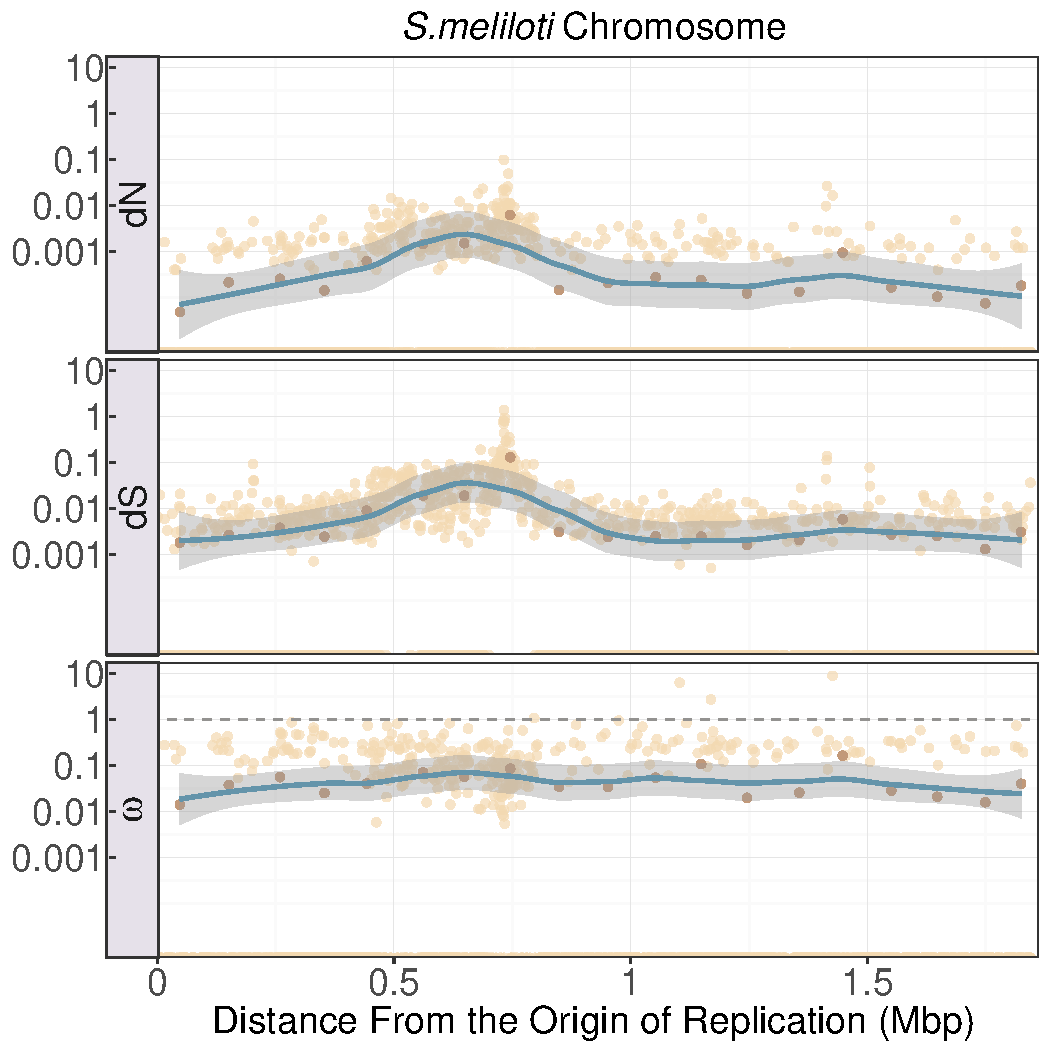
\includegraphics[width=\textwidth]{./figs/sinoC_dN_dS_omega_dist_NO_OUTLIERS.pdf}
		\caption{\label{fig:sinoC_selection_no_outliers}The graph show the values of \dn, \ds, and $\omega$ along the chromosome of \smel. Distance from the origin of replication is on the x-axis beginning with the origin of replication denoted by position zero on the left, and the terminus indicated on the far right. The y-axis of the graph indicates the value of \dn, \ds, and $\omega$ found at each gene segment position of the chromosome. Outliers are included in this graph. The average \dn, \ds, and $\omega$ values for each 10,000bp regions of the replicon were calculated and represented by the dark brown points. A trend line represented in blue (using the \texttt{loess} method), was fit to these average values and the associated 95\% confidence intervals for this line is represented by the grey ribbon around the blue trend line. For a complete list zero value information, please see Table \ref{tab:selection_outliers}.}
	\end{center}
\end{figure}



\newpage
\clearpage

\printbibliography[heading=bibintoc]
\end{document}
